\subsection{Overview}
The system paradigm is client-server. In particular, there is a thin client and a fat server. 
The client contains only a presentation layer. 
The server, instead, contains both the business application logic and the data management logic. 
The system paradigm is client-server. In particular, there is a thin client and a fat server. The client contains only a presentation layer. The server, instead, contains both the business application logic and the data management logic. 
The layer of the application are:
\begin{itemize}
    \item \textbf{Presentation Layer:} it manages the presentation logic and all the interactions with the user.
    \item \textbf{Application Layer:} it manages all the functionalities of the system.
    \item \textbf{Data Layer:} it manages the access and the storage of data.
\end{itemize}

\begin{figure}[H]
    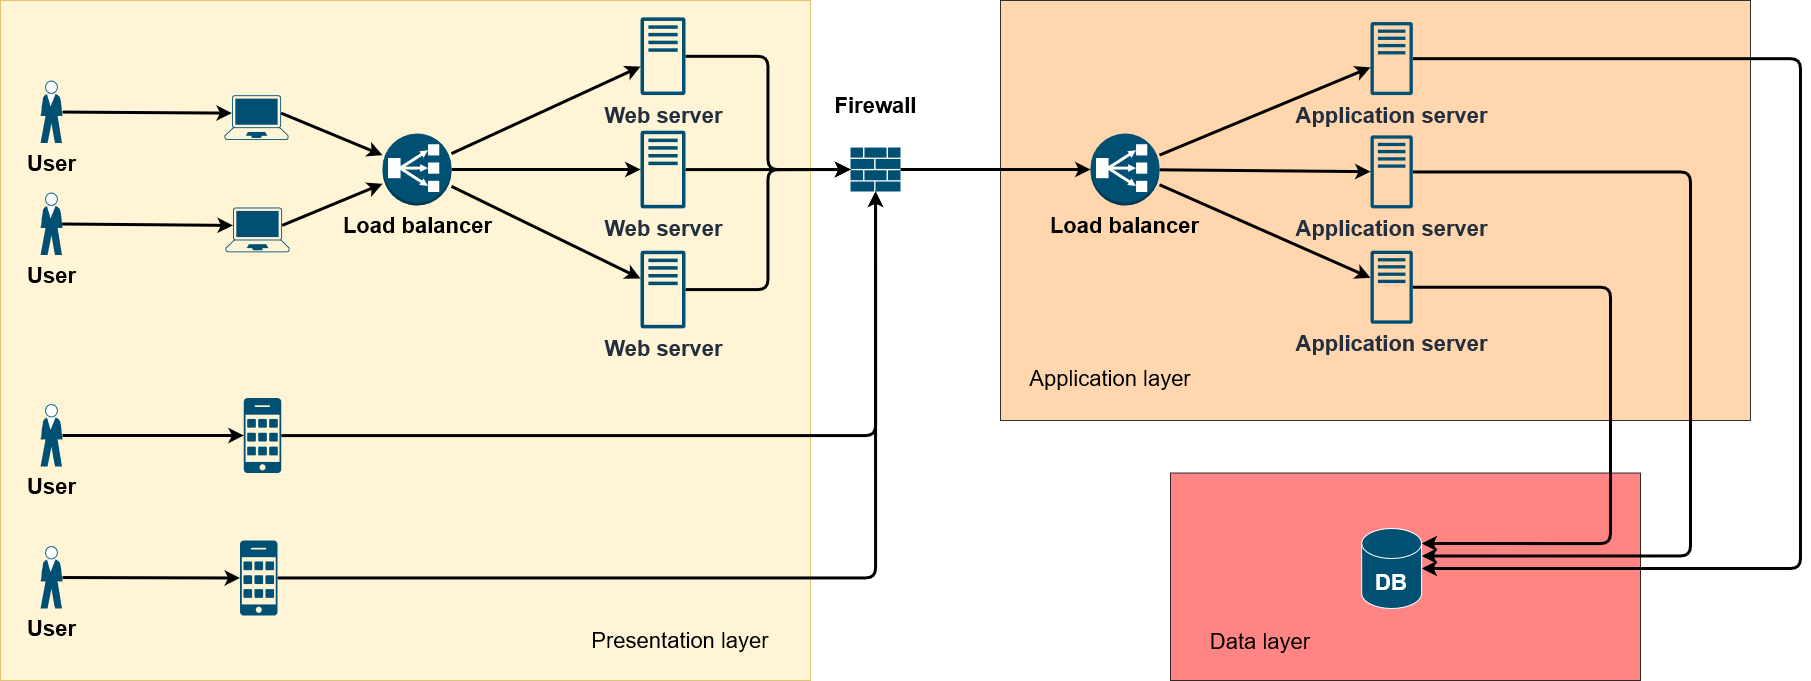
\includegraphics[width=\textwidth,height=\textheight,keepaspectratio]{Images/architectureDesignDiagram.png}
    \caption{Architecture of the application}
    \label{fig:architectue_diagram}
\end{figure}

As shown in figure \ref{fig:architectue_diagram} the application is divided into 3 layers and 4 tiers. Users can access the service
both from a mobile app or web interface. The figure shows the division of the different layers. Since the application follows the 
REST standard the servers are stateless. There will be a more precise description of the components in the following sections.

\subsection{Component View}
\begin{figure}[H]
    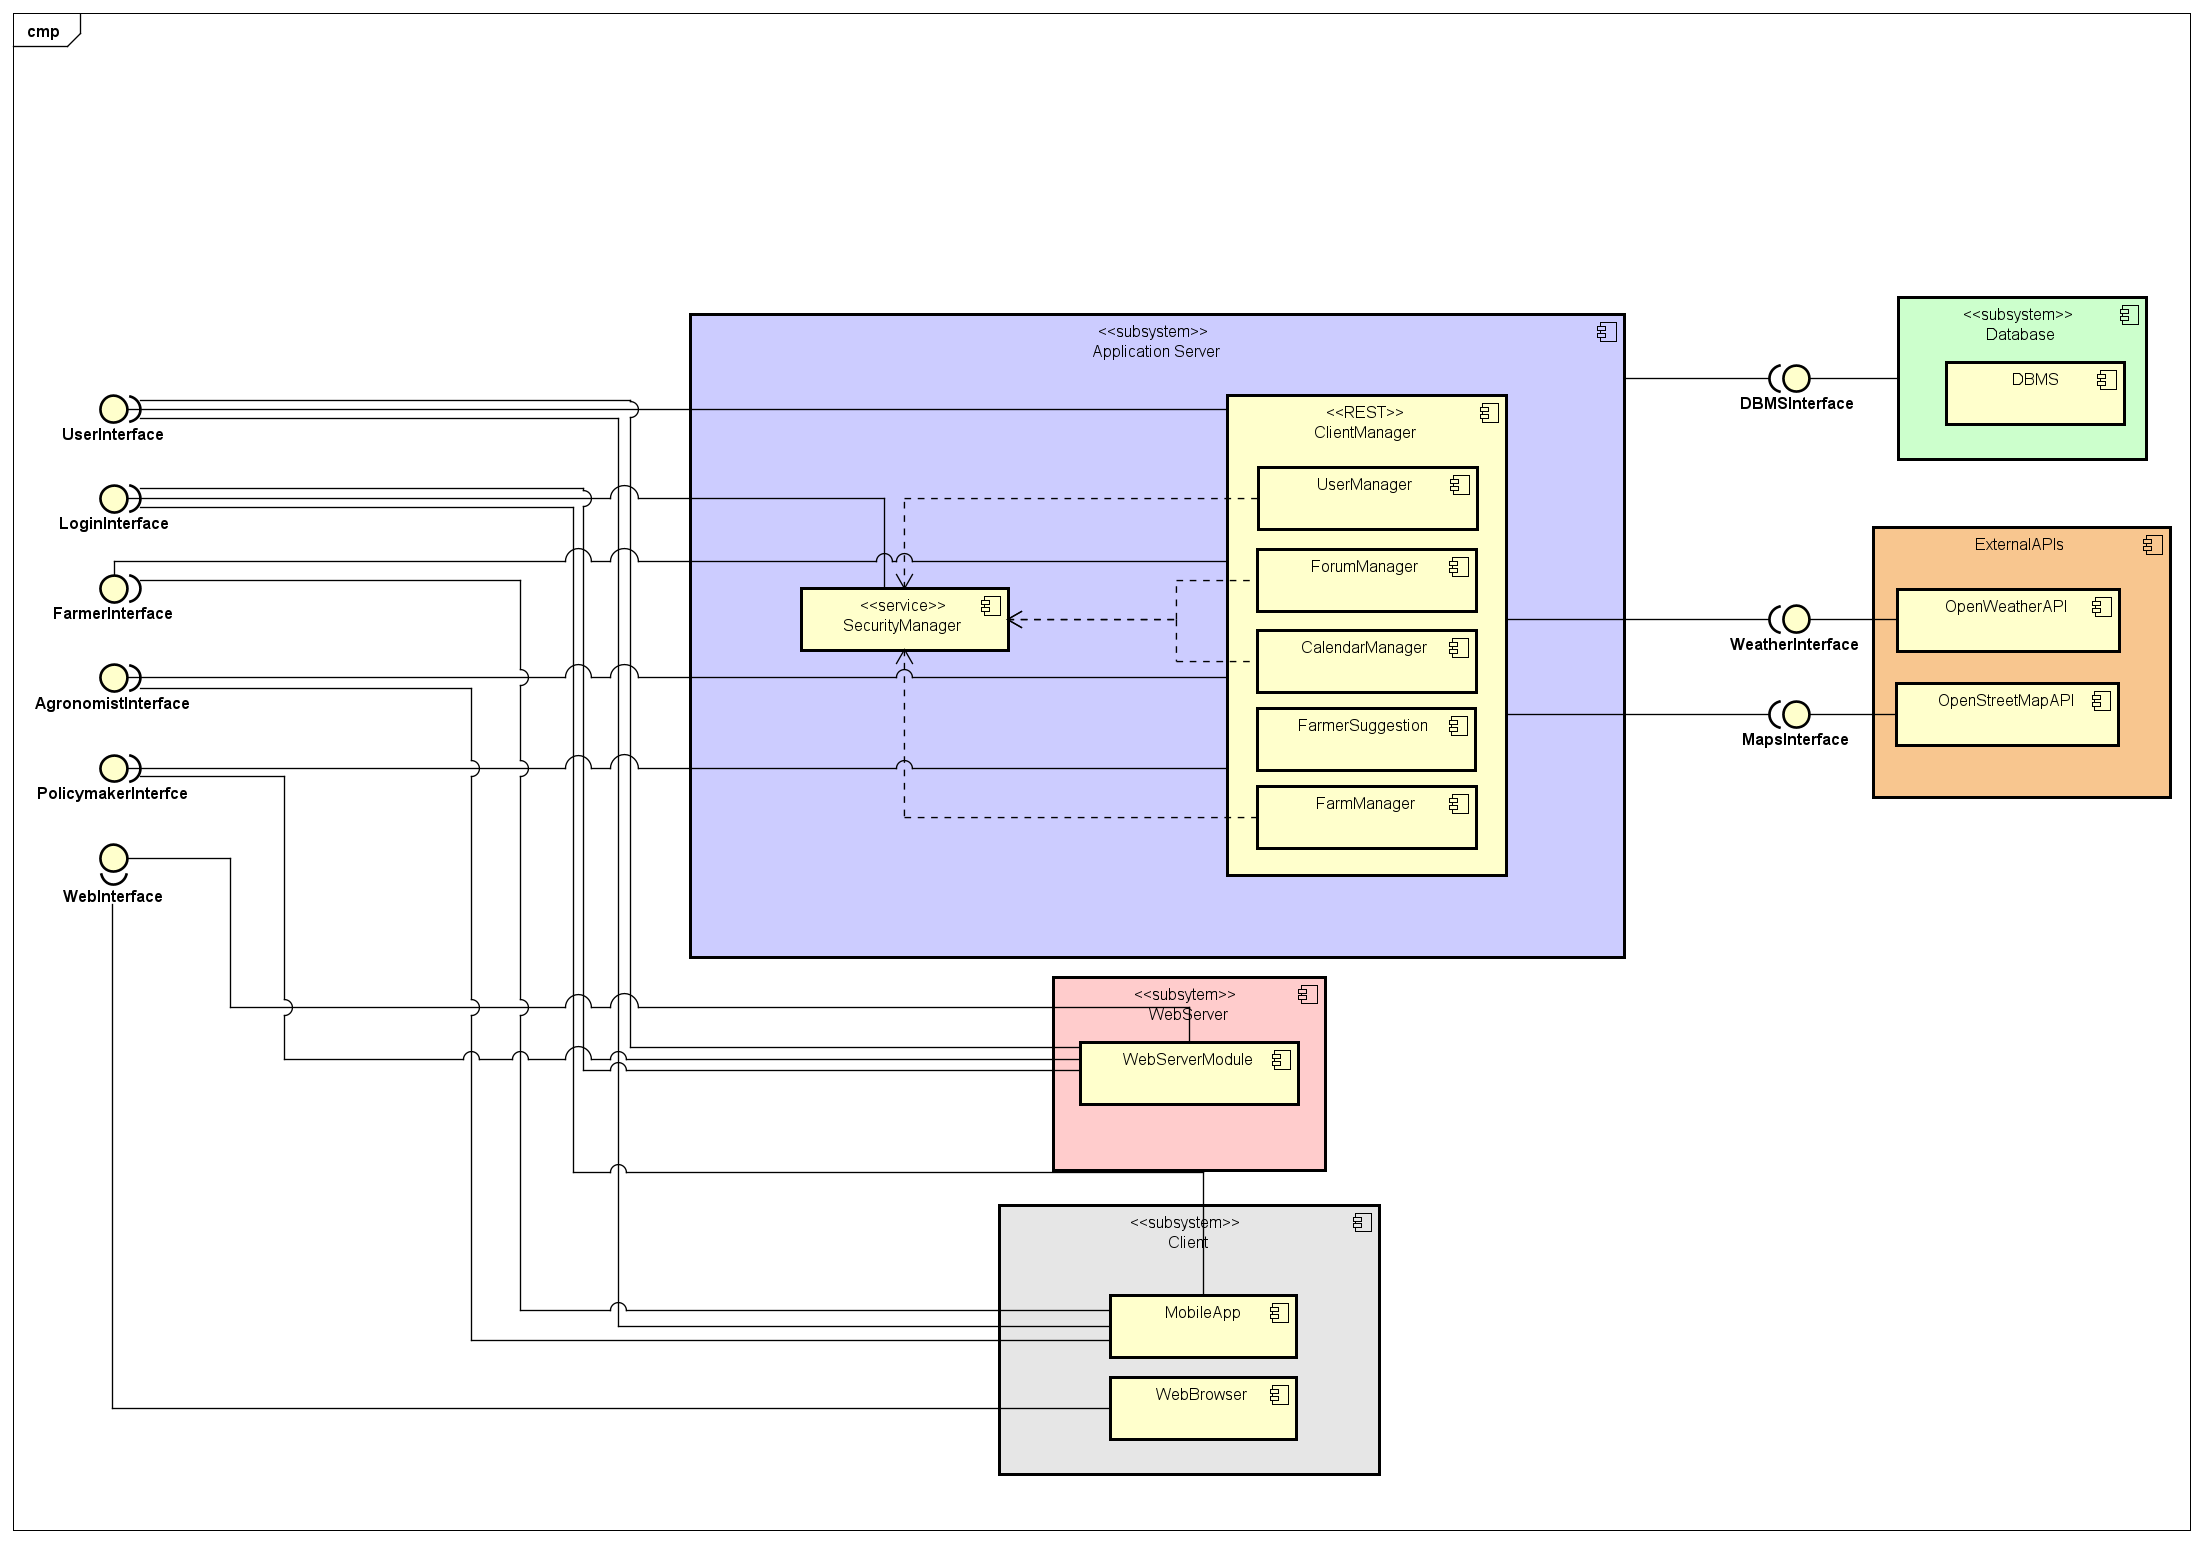
\includegraphics[width=\textwidth,height=\textheight,keepaspectratio]{Images/ComponentDiagram.png}
    \caption{Component Diagram}
    \label{fig:component_diagram}
\end{figure}

Figure \ref{fig:component_diagram}  represents in detail the layers described before. The web server has the function to
route the browser requests to the application server and send back its responses.

\begin{itemize}
    \item \textbf{Client Manager}\\
        This module handles all the requests made by the client. In the beginning,
        when the client is not logged in, the module offers (through
        the user manager) a loginInterface that allows the client to register and log in. After the login the module
        provide an interface based on the role of the user: FarmInterface for the farmer, AgronomistInterface for the agronomist,
        PolicymakerInterface for the policymaker.

    \item \textbf{User Manager}\\
        This module provides all the functionalities needed to manage the user. It includes signup and login as well as role checking 
        operation and information retrieving.
           
    \item \textbf{Forum Manager}\\
        This module provides all the functionalities through the ForumInterface for managing and using the forum. 
        It includes operations for creating and replying to a discussion on the forum.

    \item \textbf{Calendar Manager}\\
        This Module provides all the functionalities needed for the Agronomist to manage his calendar. In particular, it provides
        through, the AgronomistInterface, the possibility to add or remove an appointment, to confirm the daily plan and to check
        that each farm has at least two visits per year.

    \item \textbf{Farmer Suggestion}\\
        This module handles the creation and delivery of personalized suggestions to the Farmer. 

    \item \textbf{Farm Manager}\\
        This module provides to the Farmer all the functionalities for giving information about their farm. 
        It provides the possibility to add information about the harvest and to request help from the Agronomist.

    \item \textbf{Security Manager}\\
        This module handles all the security issues.
\end{itemize}

\newpage
\subsection{Deployment diagram}
\begin{figure}[H]
    \begin{center}
        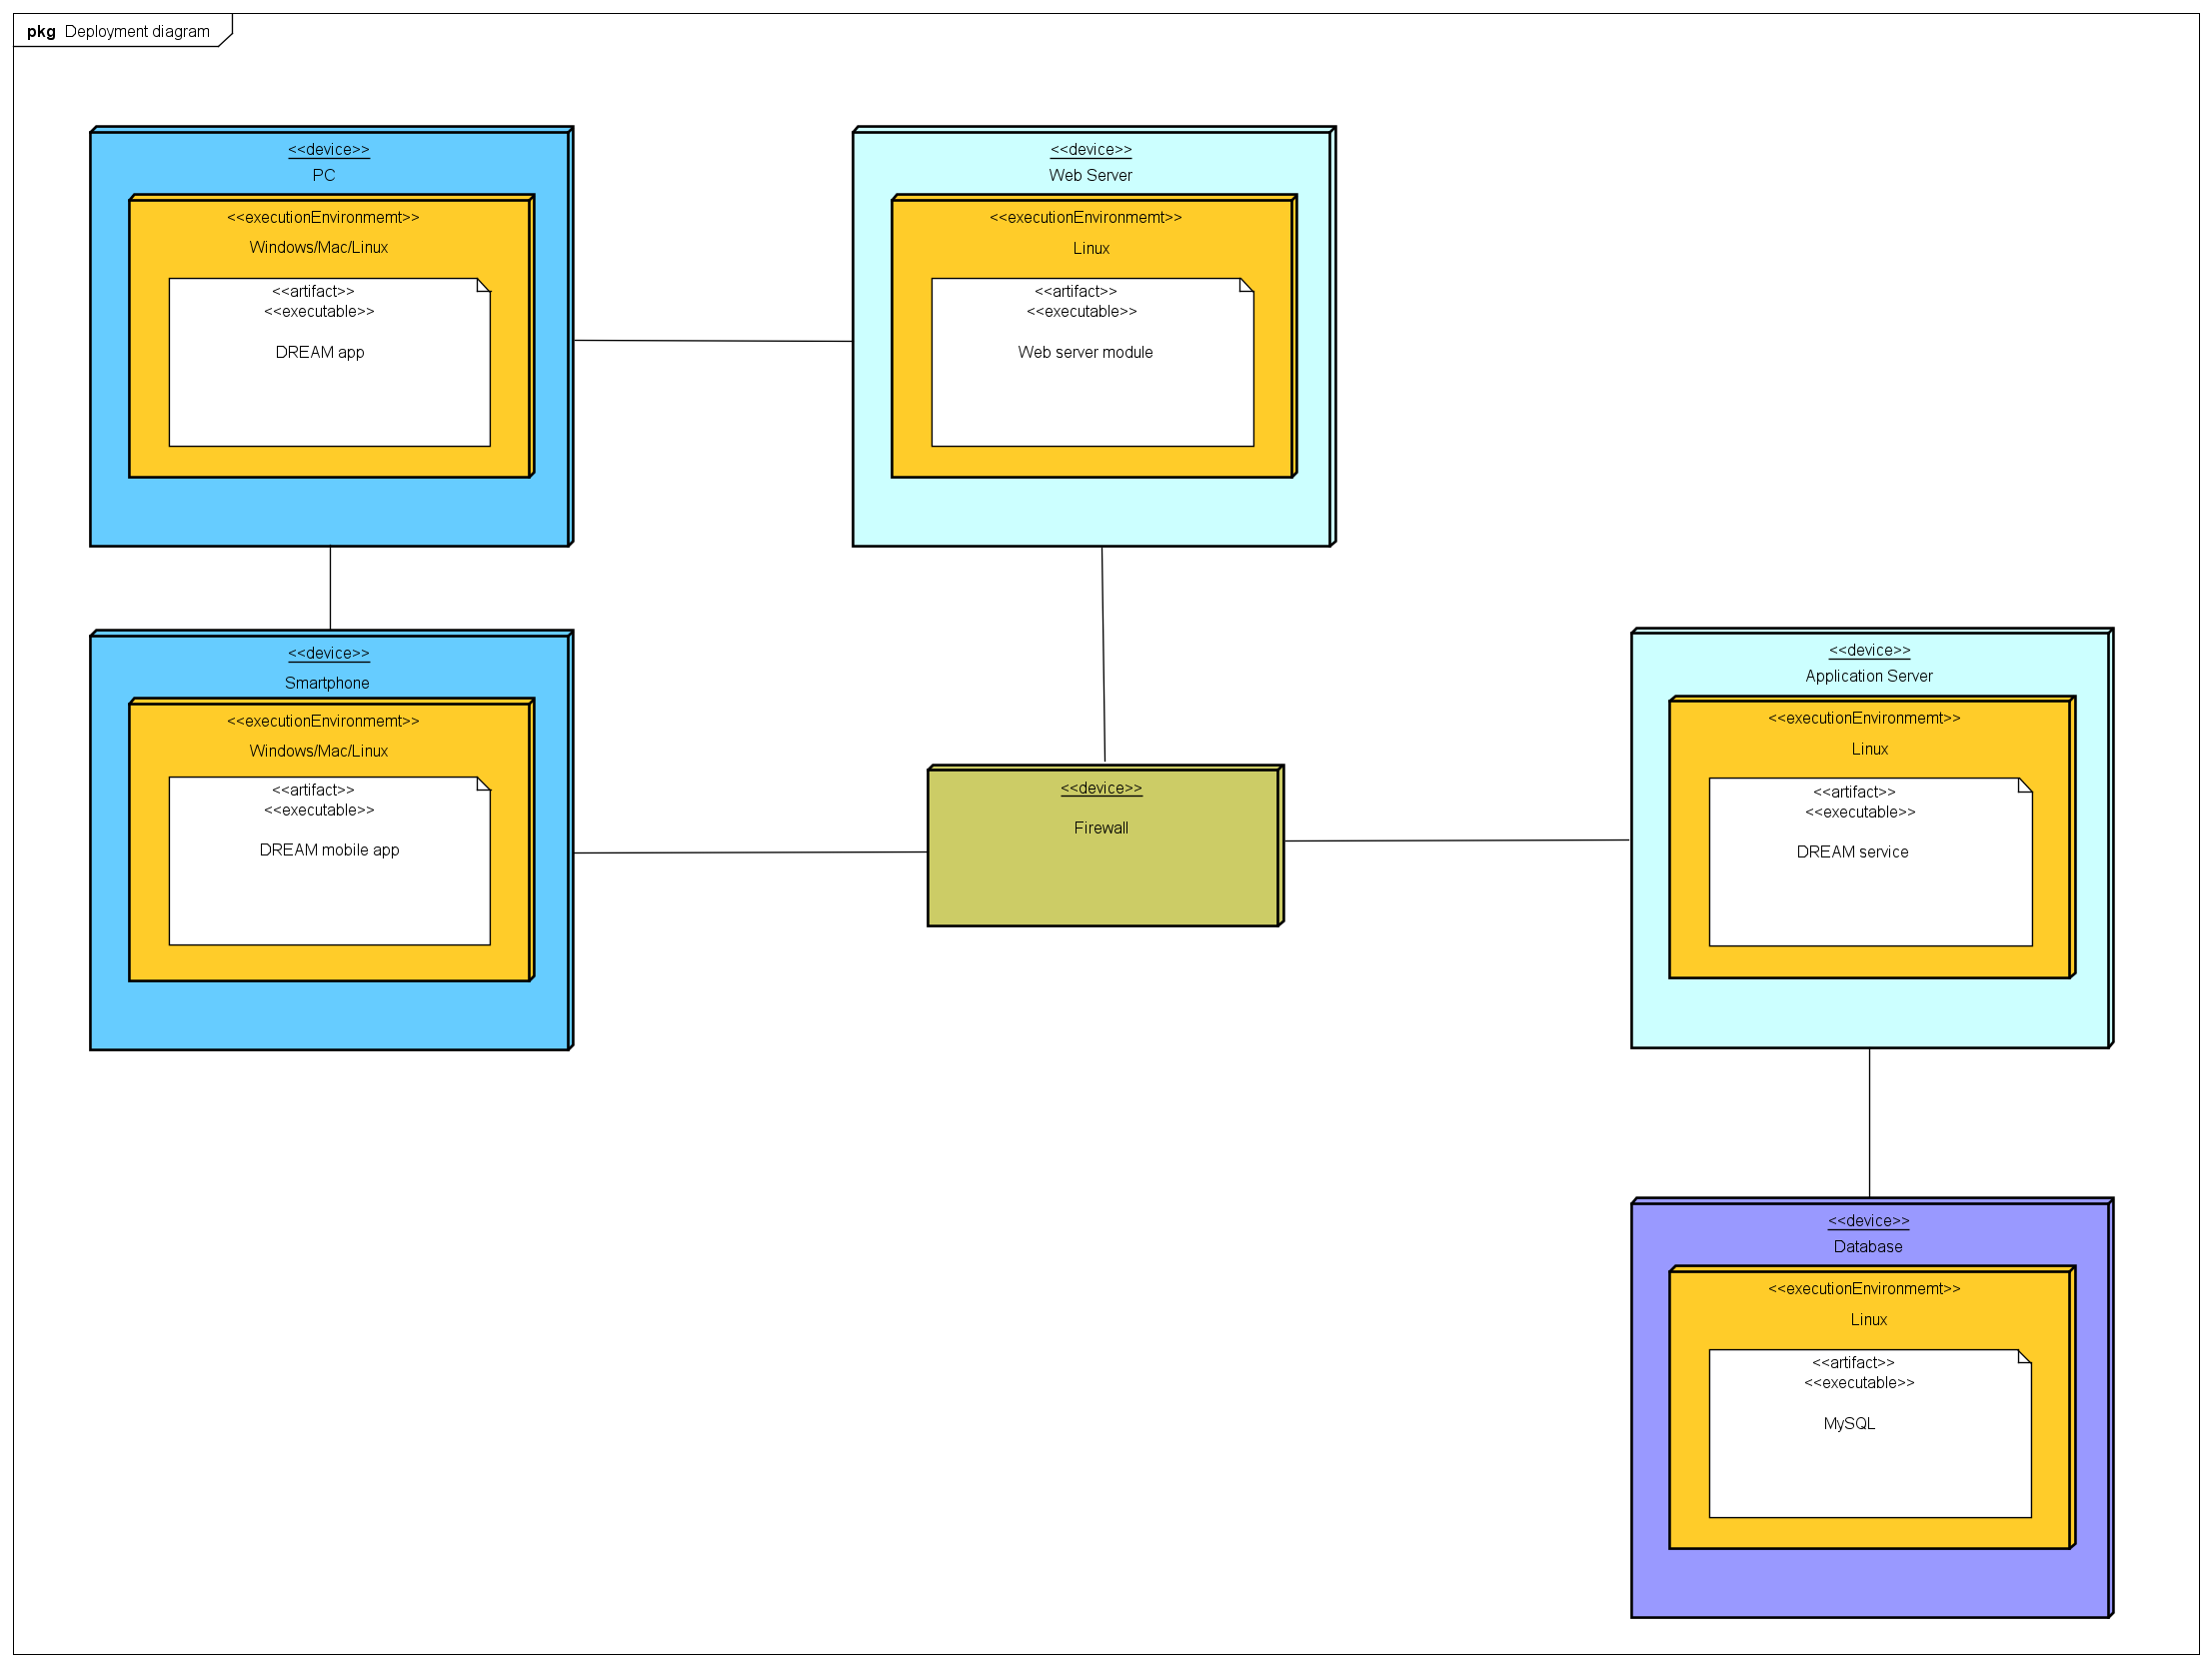
\includegraphics[width=\textwidth]{Images/DeploymentDiagram.png}
        \caption{Deployment Diagram}
    \end{center}
\end{figure}

The deployment diagram in figure shows the needed components for correct system behavior.
Each device owns its Operating System where the software runs. Firewall ensures application security.
\newline The tiers in the image are the following:
\begin{itemize}
    \item \textbf{Tier 1:} it is the client machine, which can be a computer with a web browser or the mobile
    application.
    \item \textbf{Tier 2:} includes the replicated web servers, which do not execute any business logic, but simply receive
    requests from the client, route them to the application servers and serve an HTML back to the client.
    \item \textbf{Tier 3:} it includes the application servers that contain the whole application layer and communicate to the data tier.
    \item \textbf{Tier 4:} it contains the DBMS servers that store and manage data, according to the instructions given by the application servers.
\end{itemize}

\newpage

\subsection{Runtime View}
The following sequence diagrams represent the runtime view, for every possible operation in DREAM, 
from the mobile app's perspective (for agronomists and farmers) and the web browser's perspective (for policymakers).\\
Every interface use REST API through HTTP GET and POST.

\subsubsection{Sign Up}

\begin{figure}[H]
    \begin{center}
        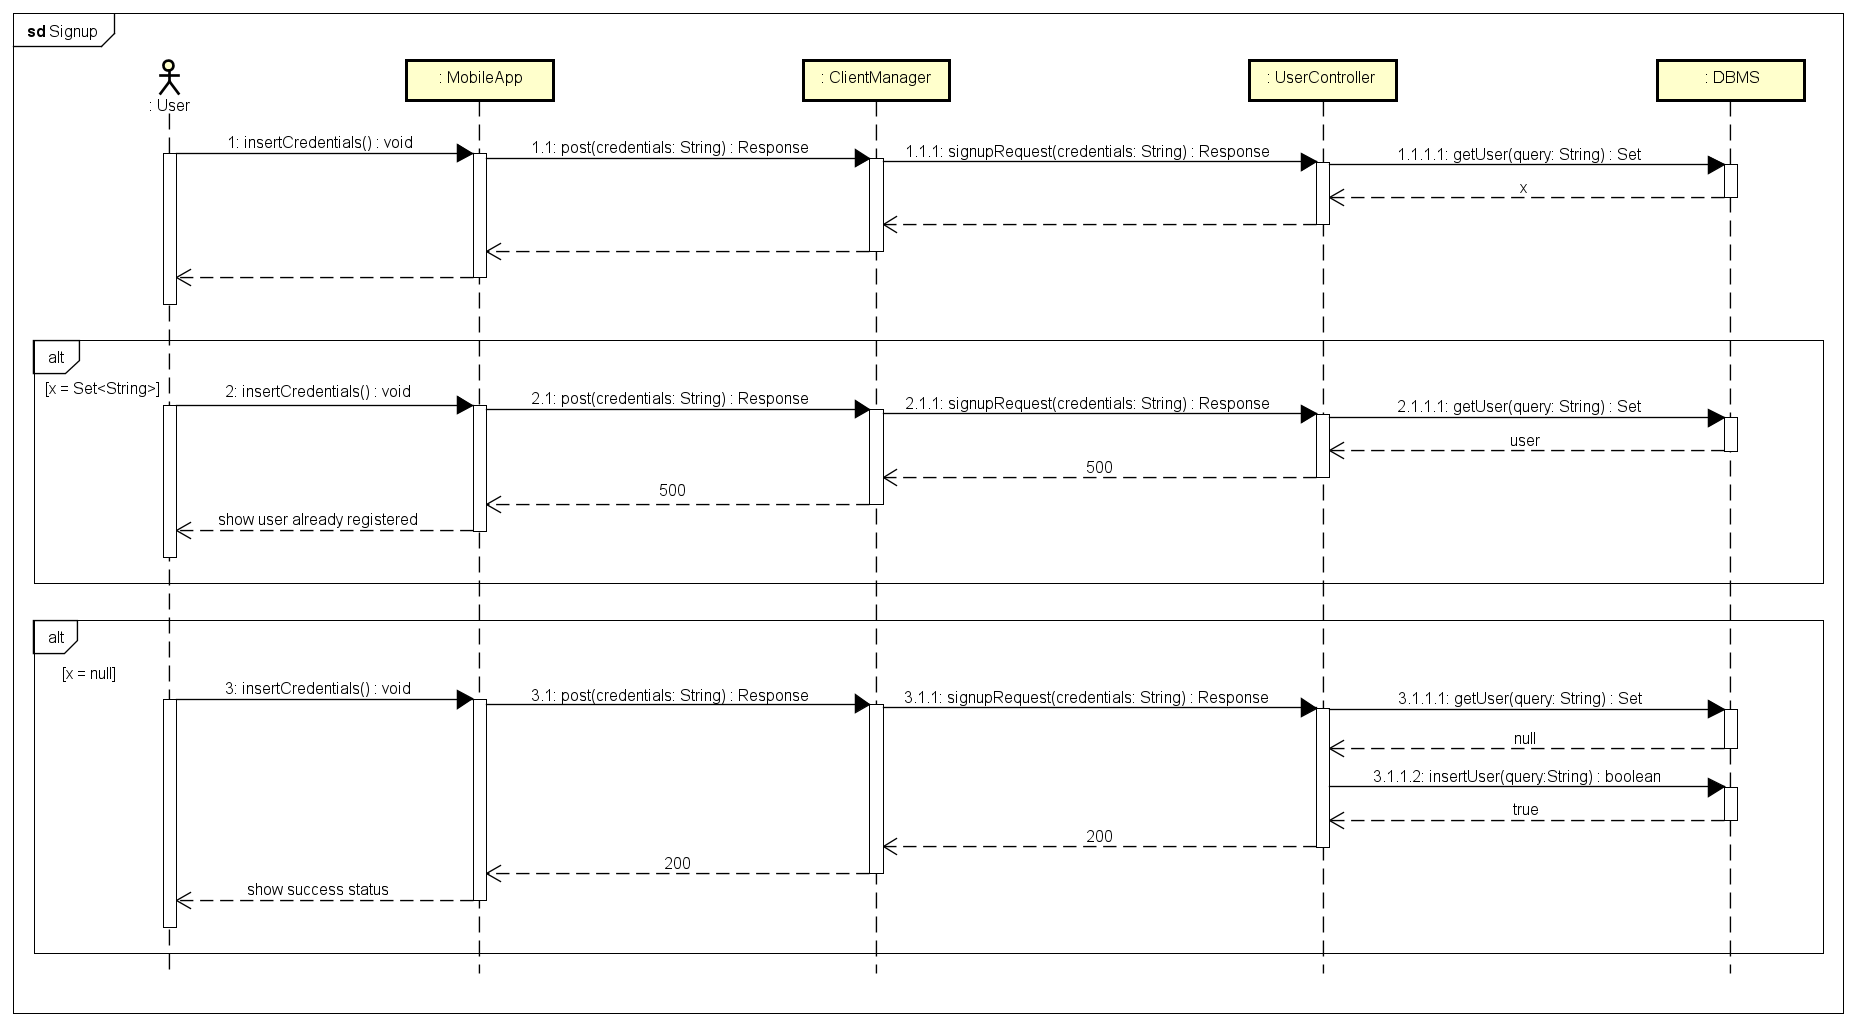
\includegraphics[width=\textwidth]{Images/SequenceDiagrams/SignupDD.png}
    \end{center}
\end{figure}

This diagram represents the process of signing up a user through two possible situations: 
\begin{itemize}
    \item User is already registered;
    \item User isn't already registered.
\end{itemize}
After the User inserts his credentials and the data are transmitted to the database, 
they are analyzed and we will have the two separate ways.\\
If these credentials are already present in the database, the UserController 
sends a 500 response's status code, warning the User that a previous registration with these data exists.\\
Otherwise, if the credentials aren't present in the DBMS, the UserController inserts the User 
into the database and sends a 200 response's status code, informing the User that the registration was successful.


\newpage
\subsubsection{Login}

\begin{figure}[H]
    \begin{center}
        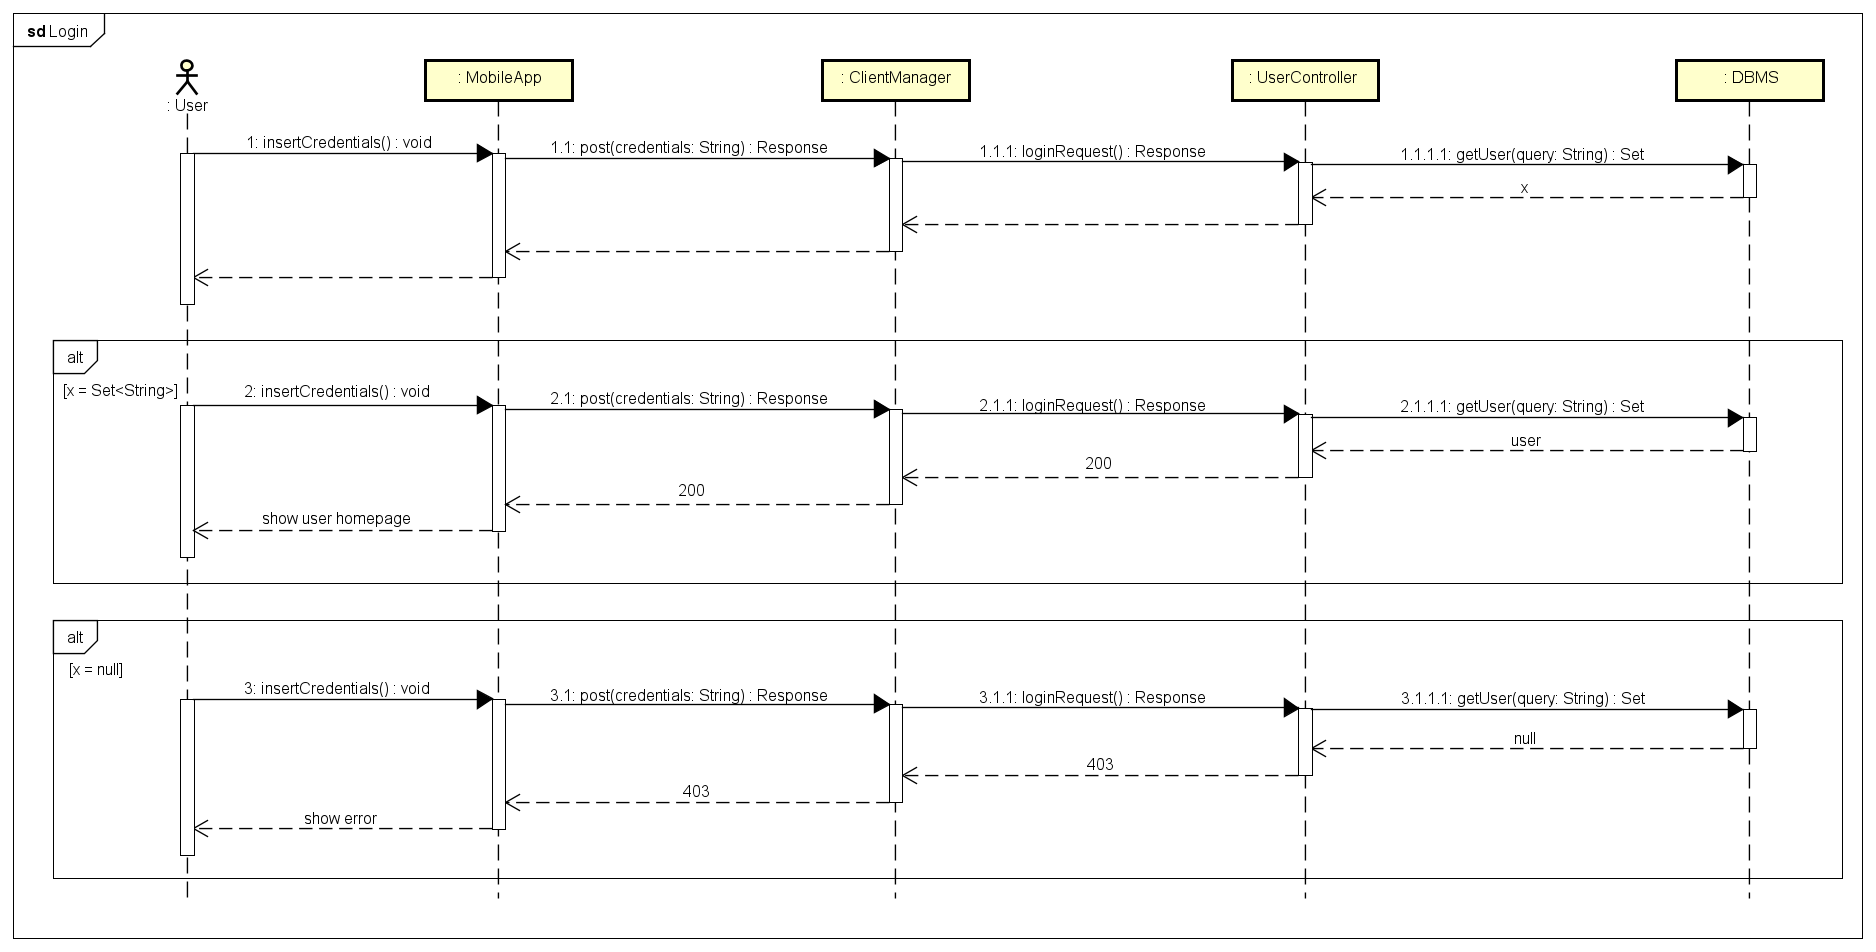
\includegraphics[width=\textwidth]{Images/SequenceDiagrams/LoginDD.png}
    \end{center}
\end{figure}

This diagram represents the process of login of a User and has the same two ways as the process of signing up:
\begin{itemize}
    \item User is already registered;
    \item User isn't already registered.
\end{itemize}
After the user enters his credentials and these are analyzed by the database, 
the two paths are opposite with respect to the registration case.\\
If the user is already present in the database, the UserController sends a 
200 response's status and the User is taken to the homepage.\\
If the user is not already present in the database, the UserController sends 403 responses's status, 
warning the User that a previous registration with these data doesn't exist.


\newpage
\subsubsection{Insert Area}

\begin{figure}[H]
    \begin{center}
        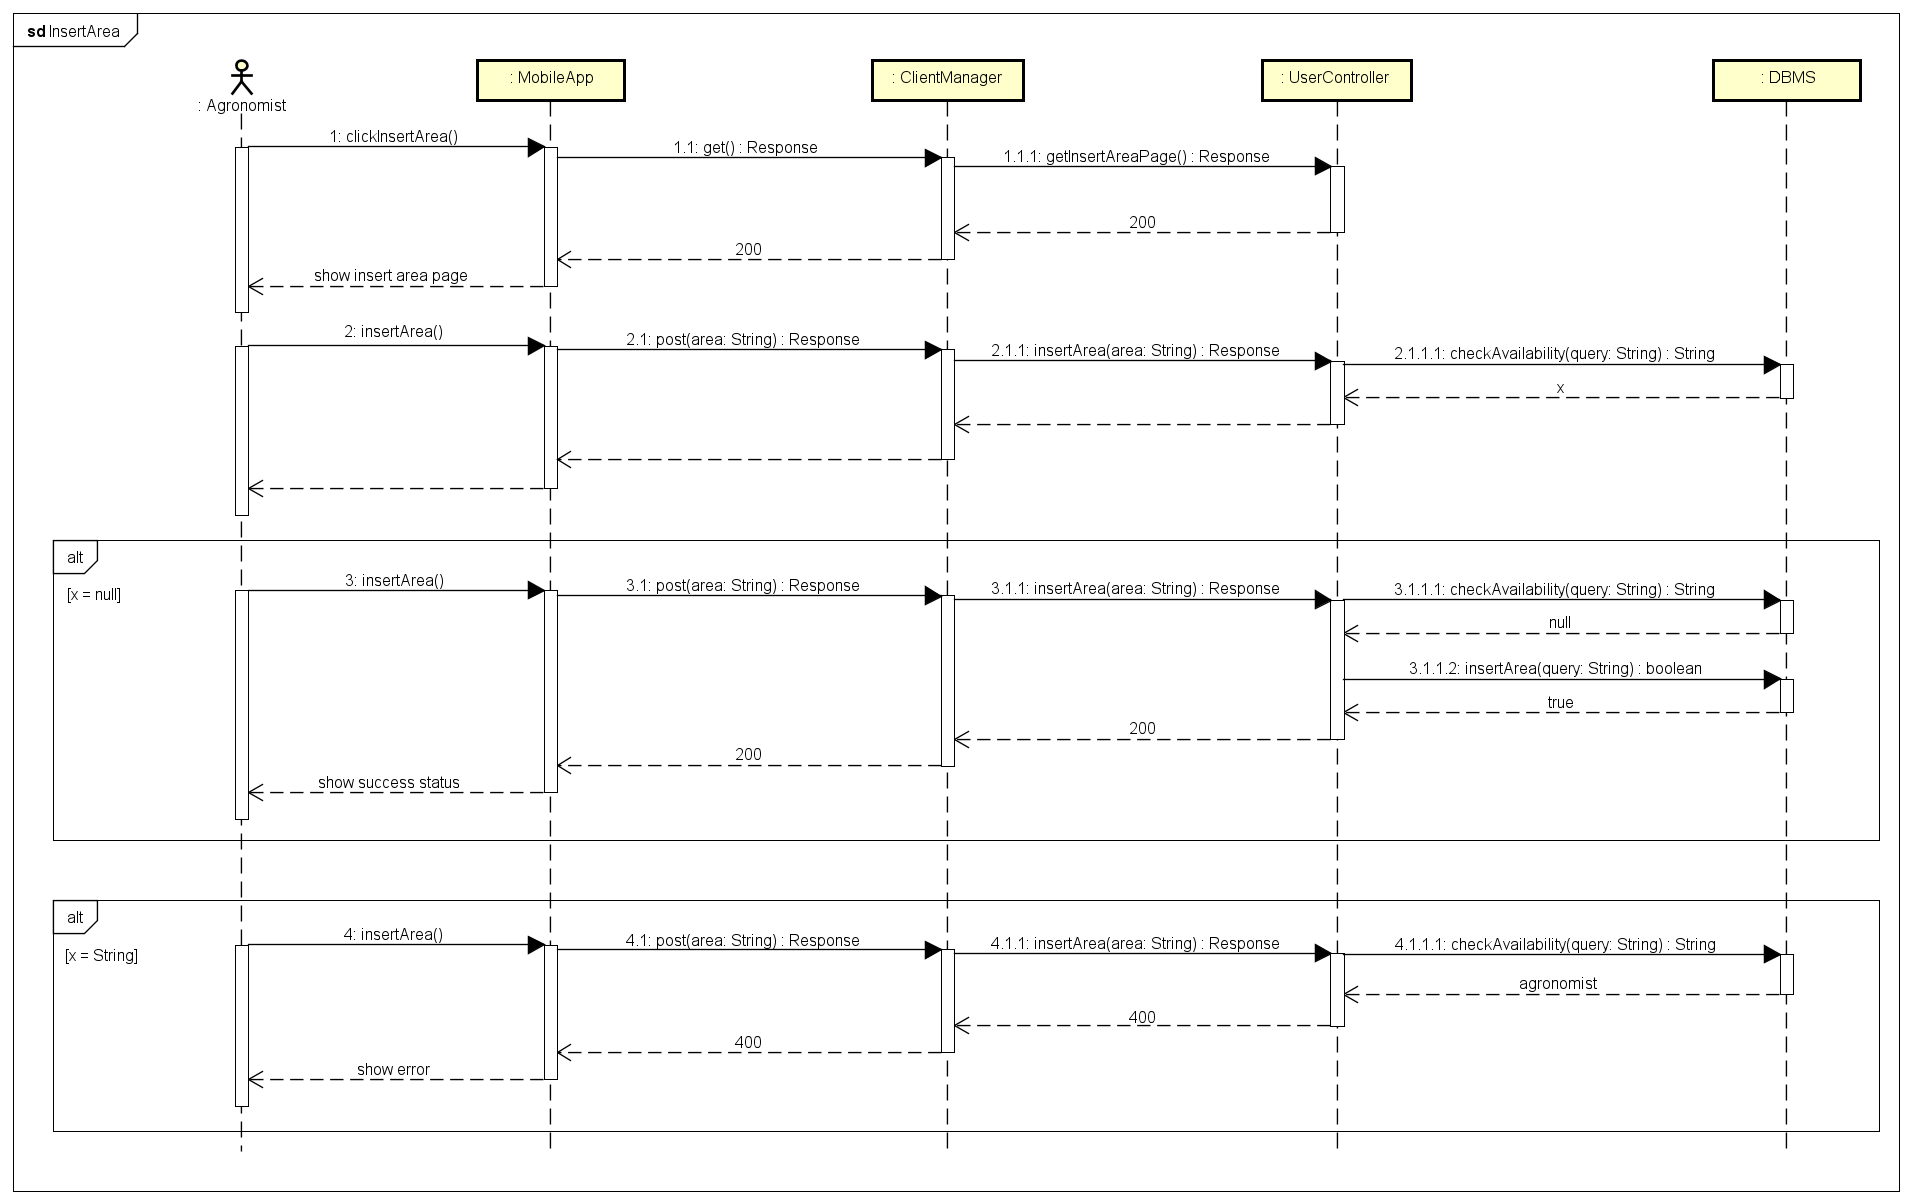
\includegraphics[width=\textwidth]{Images/SequenceDiagrams/InsertAreaDD.png}
    \end{center}
\end{figure}

This sequence diagram represents an operation that could be done only by agronomists.\\
After the user inserts the area he is responsible for, the UserController checks in the 
DBMS if there is already a registered agronomist responsible for the same area that the User inserted.\\
If there isn't a registered agronomist, the UserController inserts the area in the DBMS and sends a 200 
response's status code to the User; otherwise sends a 400 response's status code to the User.


\newpage
\subsubsection{Add appointment}

\begin{figure}[H]
    \begin{center}
        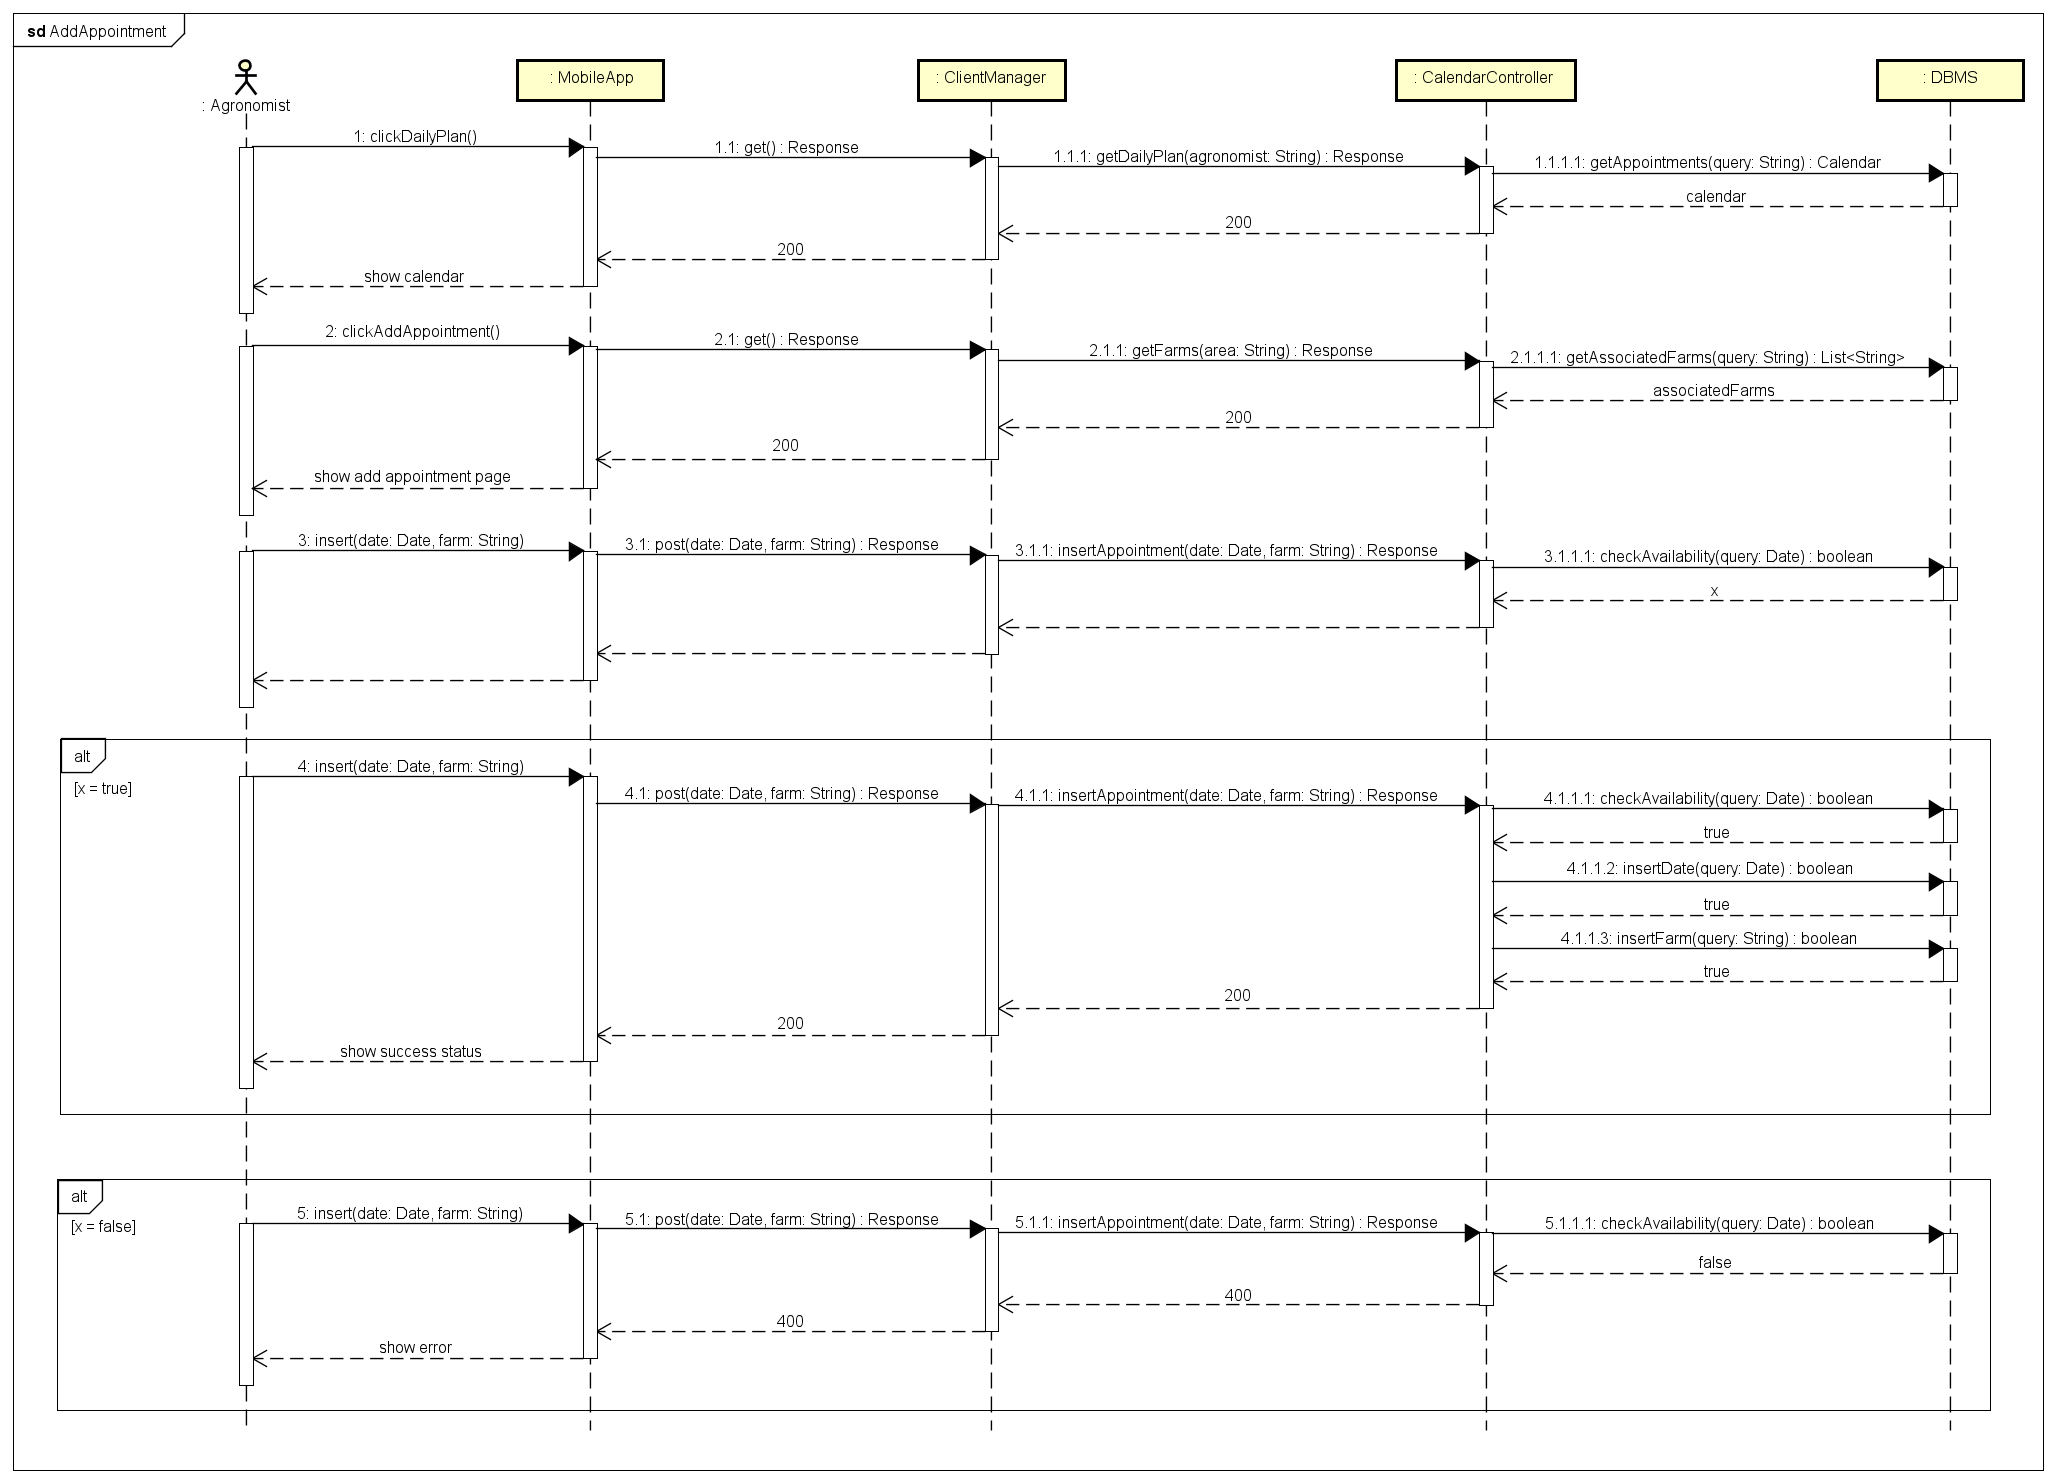
\includegraphics[width=\textwidth]{Images/SequenceDiagrams/AddAppointmentDD.png}
    \end{center}
\end{figure}

This sequence diagram shows the steps that an agronomist has to do for adding an appointment.\\
After checking the daily plan, the agronomist can press on "ADD" button and specify the farm and the date 
of the appointment that he wants to make.\\
The CalendarController query the DBMS to check if the selected date is available and here we have two different ways.\\
If the date is available, the CalendarController adds the appointment in the DBMS and sends a 200 response's status code to the User;
otherwise, the CalendarController sends a 400 response's status code to the User.


\newpage
\subsubsection{Answer on the Forum}

\begin{figure}[H]
    \begin{center}
        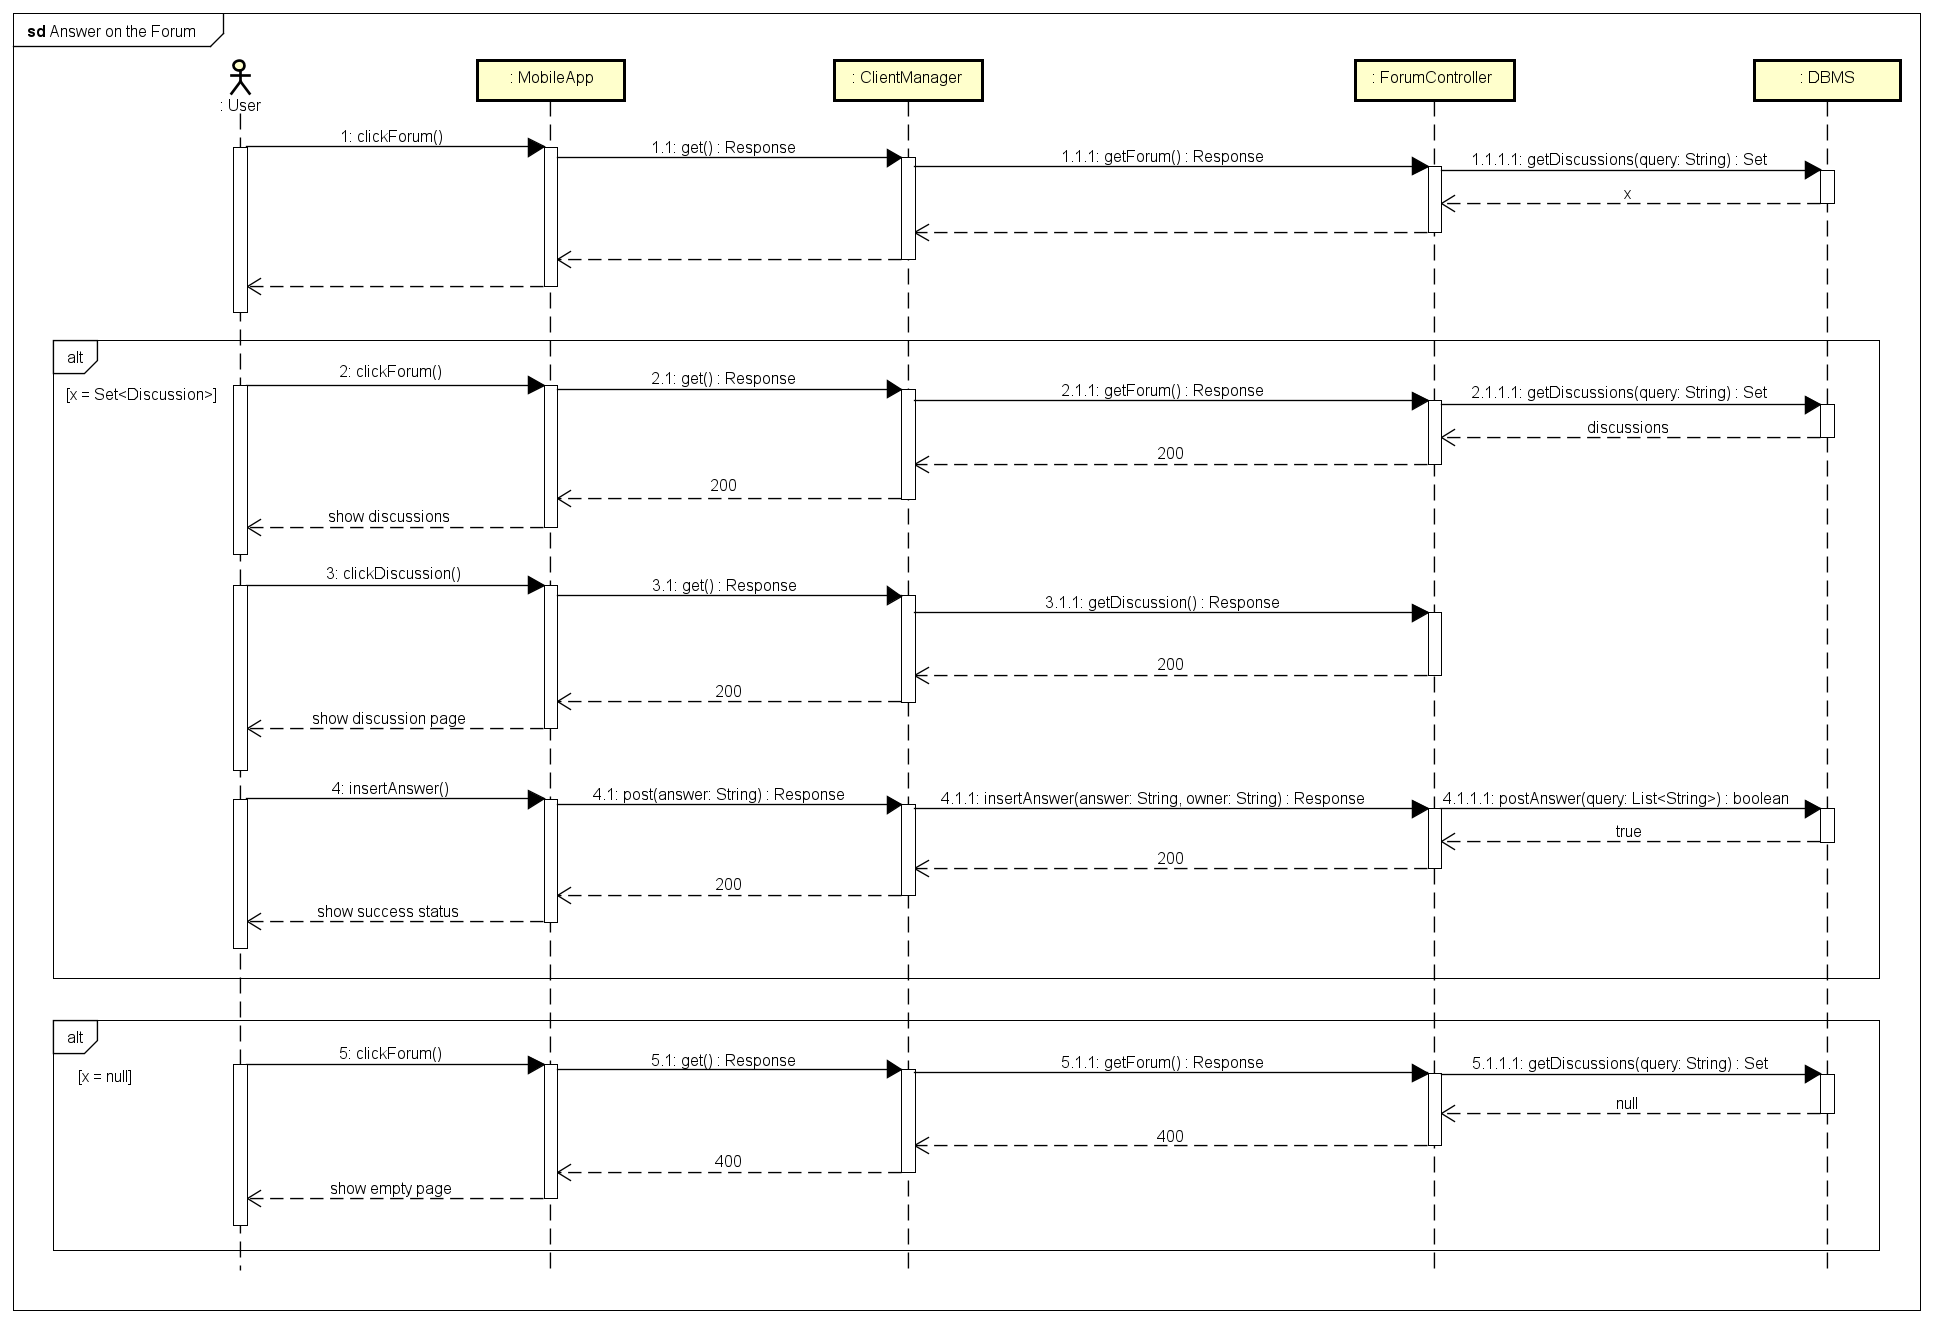
\includegraphics[width=\textwidth]{Images/SequenceDiagrams/AnswerForumDD.png}
    \end{center}
\end{figure}

This sequence diagram represents an operation that could be done by an agronomist or a farmer.\\
The User has to press on a discussion and insert his answer. After that, the ForumController inserts the answer in the DBMS
and sends a 200 response's status code to the User.\\
The ForumController sends a 400 response's status code to the User only if there isn't an open discussion thus showing an empty page.


\newpage
\subsubsection{Check Dashboard}

\begin{figure}[H]
    \begin{center}
        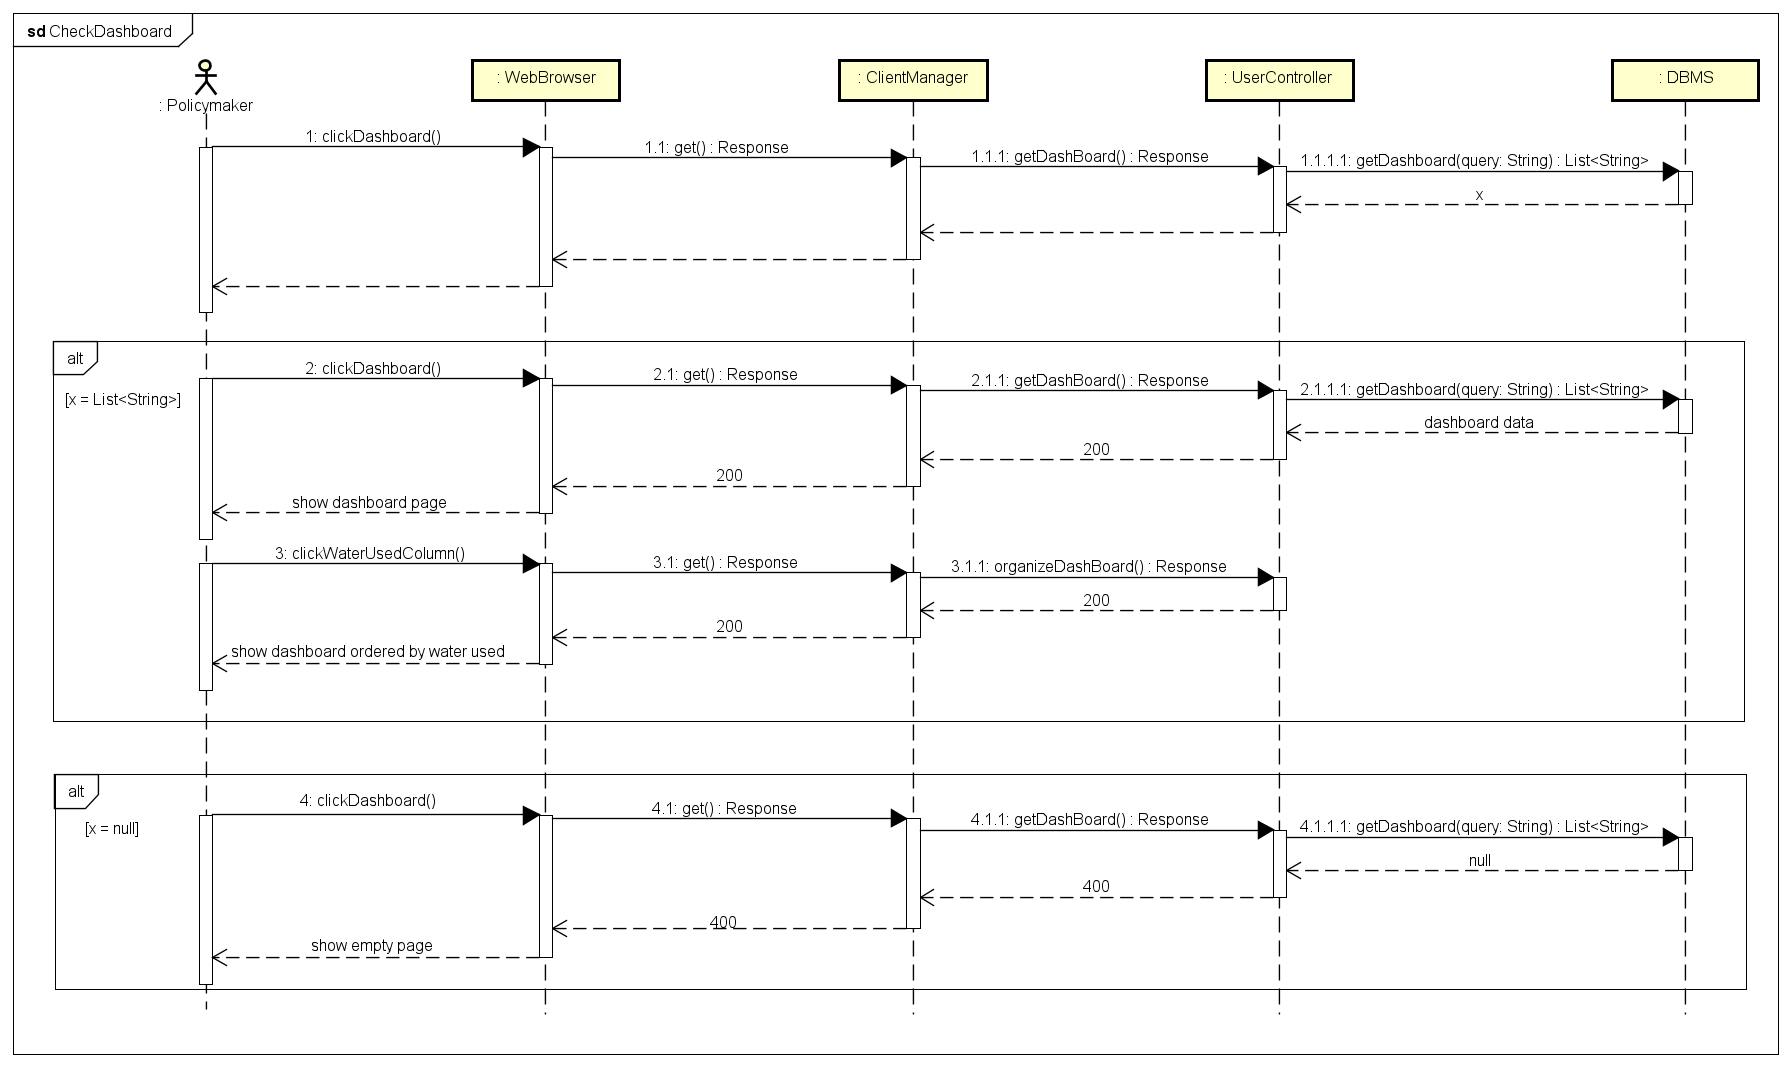
\includegraphics[width=\textwidth]{Images/SequenceDiagrams/CheckDashboardDD.png}
    \end{center}
\end{figure}

This sequence diagram represents an operation that could be done by agronomists and policymakers. 
The only difference between the operation done by these two different users is that the policymakers can check the dashboard 
of all farms, while the agronomists can check only the dashboard about the farms of the area that he is responsible for.\\
After retrieving the data from the DBMS, the UserController sends a 200 response's status code to the User and shows him the dashboard. 
The User can then reorganize the data according to one of the fields on the dashboard.\\
The UserController sends a 400 response's status code to the User only 
if there isn't data about farms in the DBMS thus showing an empty page.


\newpage
\subsubsection{Check Weather Forecasts}

\begin{figure}[H]
    \begin{center}
        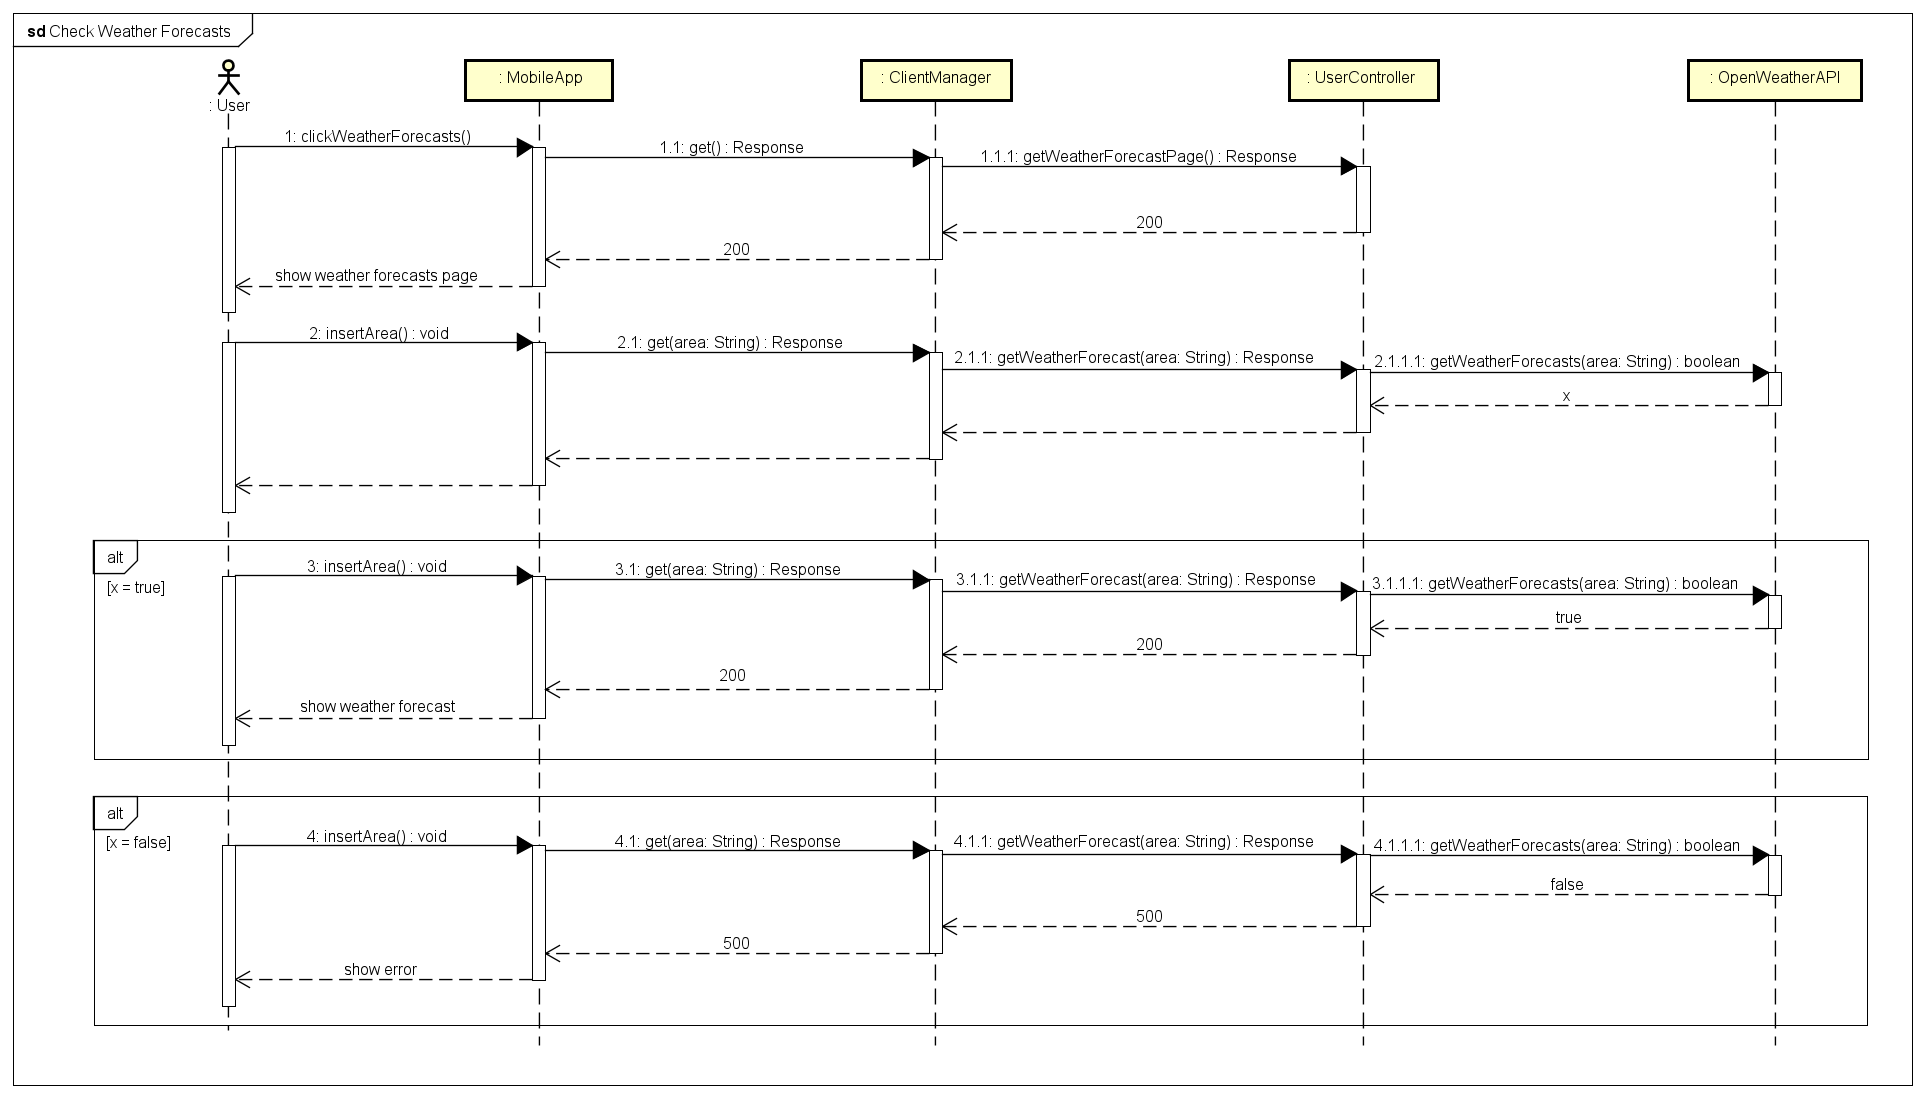
\includegraphics[width=\textwidth]{Images/SequenceDiagrams/CheckWeatherForecastsDD.png}
    \end{center}
\end{figure}

This sequence diagram represents an operation that could be done by agronomists and farmers.\\
On the Weather Forecasts page, the User has to specify the area for which he wants to know the weather forecast.\\
After that, the UserController query the OpenWeatherAPI and, if the inserted area exists, 
the Controller sends a 200 response's status code to the User and shows him the weather forecast.\\
In case of the inserted area doesn't exist, the OpenWeatherAPI responds to the request 
with "false" and the UserController sends a 500 response's status code to the User.


\newpage
\subsubsection{Help Request}

\begin{figure}[H]
    \begin{center}
        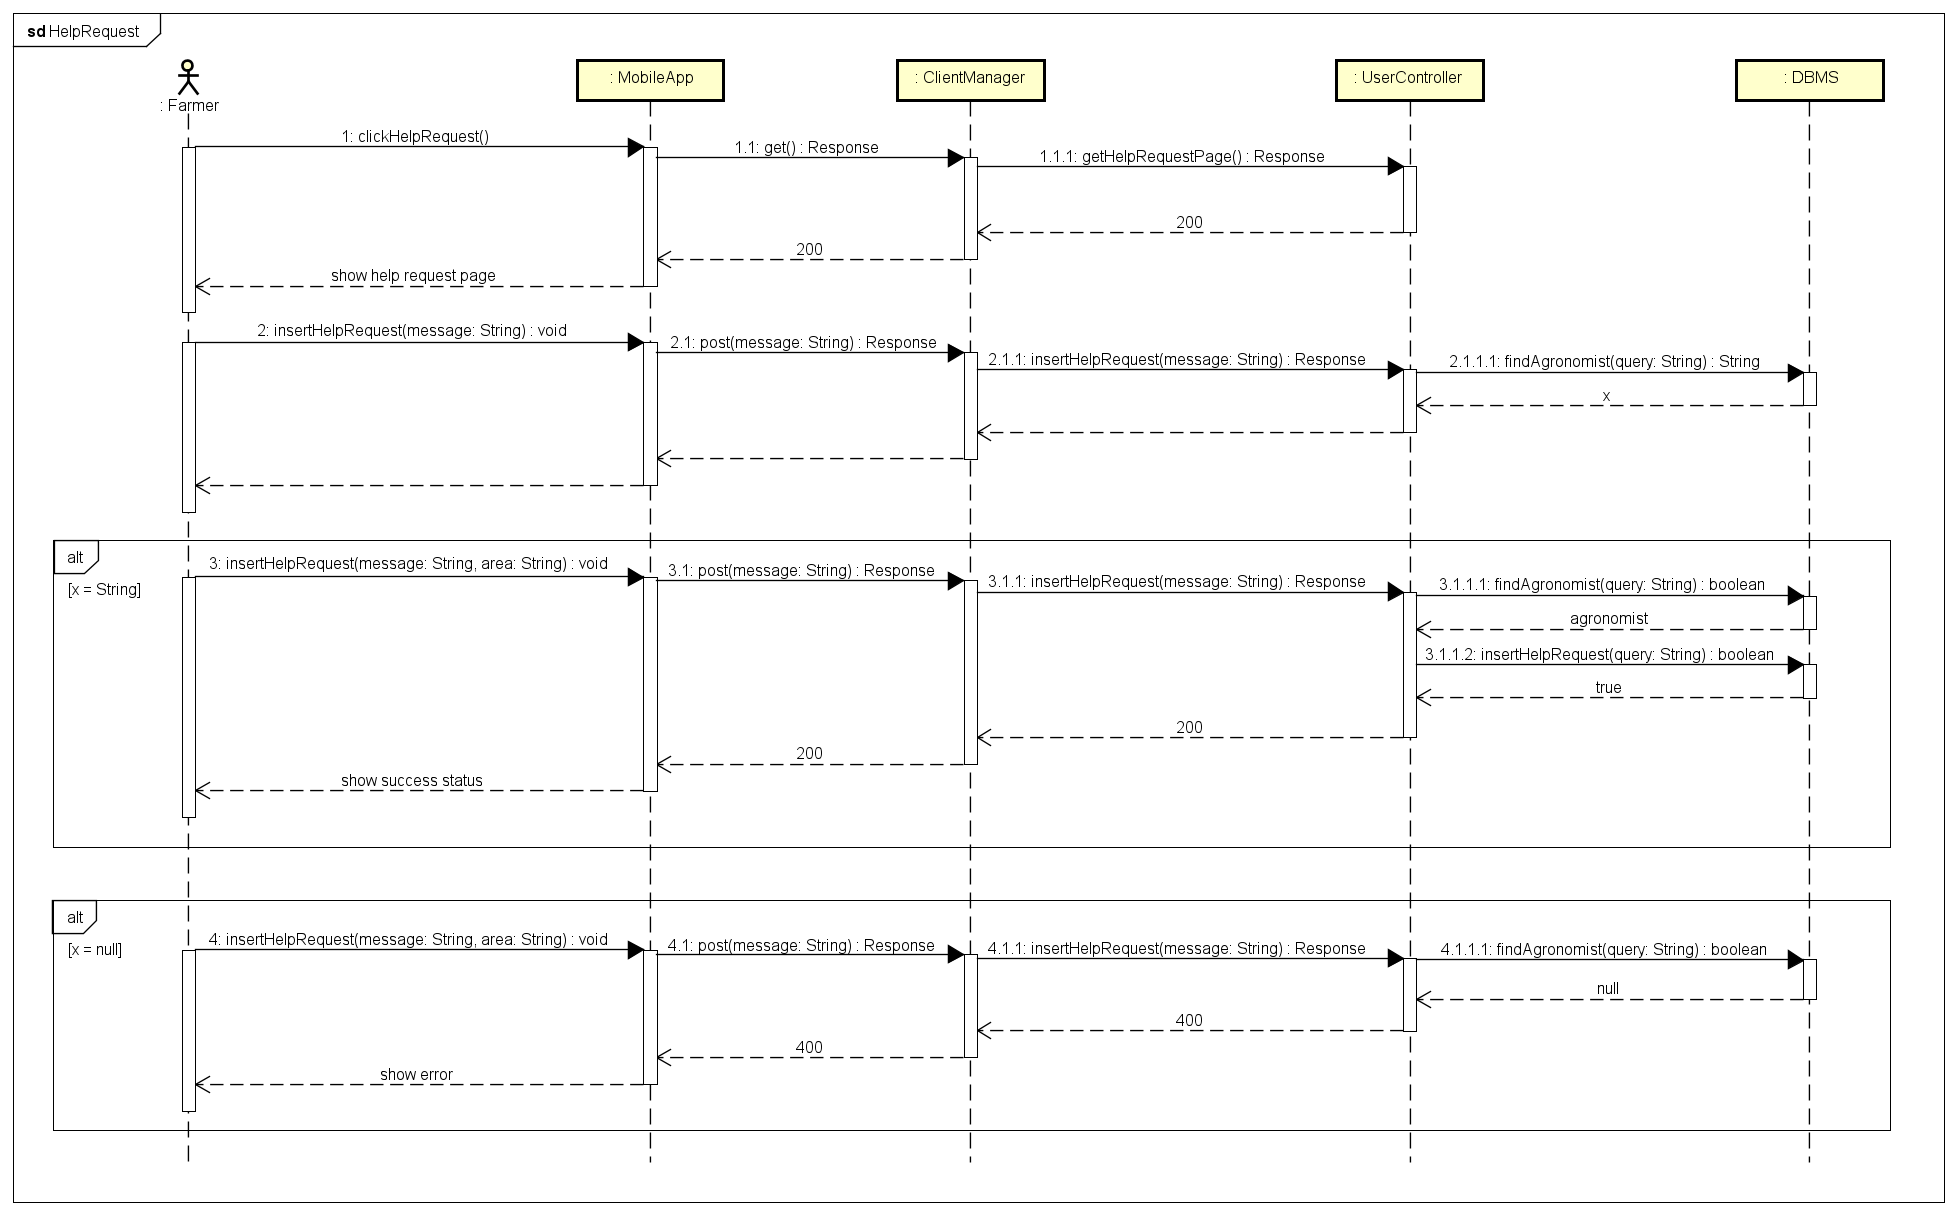
\includegraphics[width=\textwidth]{Images/SequenceDiagrams/HelpRequestDD.png}
    \end{center}
\end{figure}

This sequence diagram represents how the privately help requests by farmers occur.\\
After the farmer describes his problem, the UserController checks in the DBMS if there 
is a registered agronomist responsible for the same area where the User's farm is located.\\
If there is a registered agronomist, the UserController inserts the help request in the DBMS and sends 
a 200 response's status code to the User; otherwise sends a 400 response's status code to the User.


\newpage
\subsubsection{Reply Help Request}

\begin{figure}[H]
    \begin{center}
        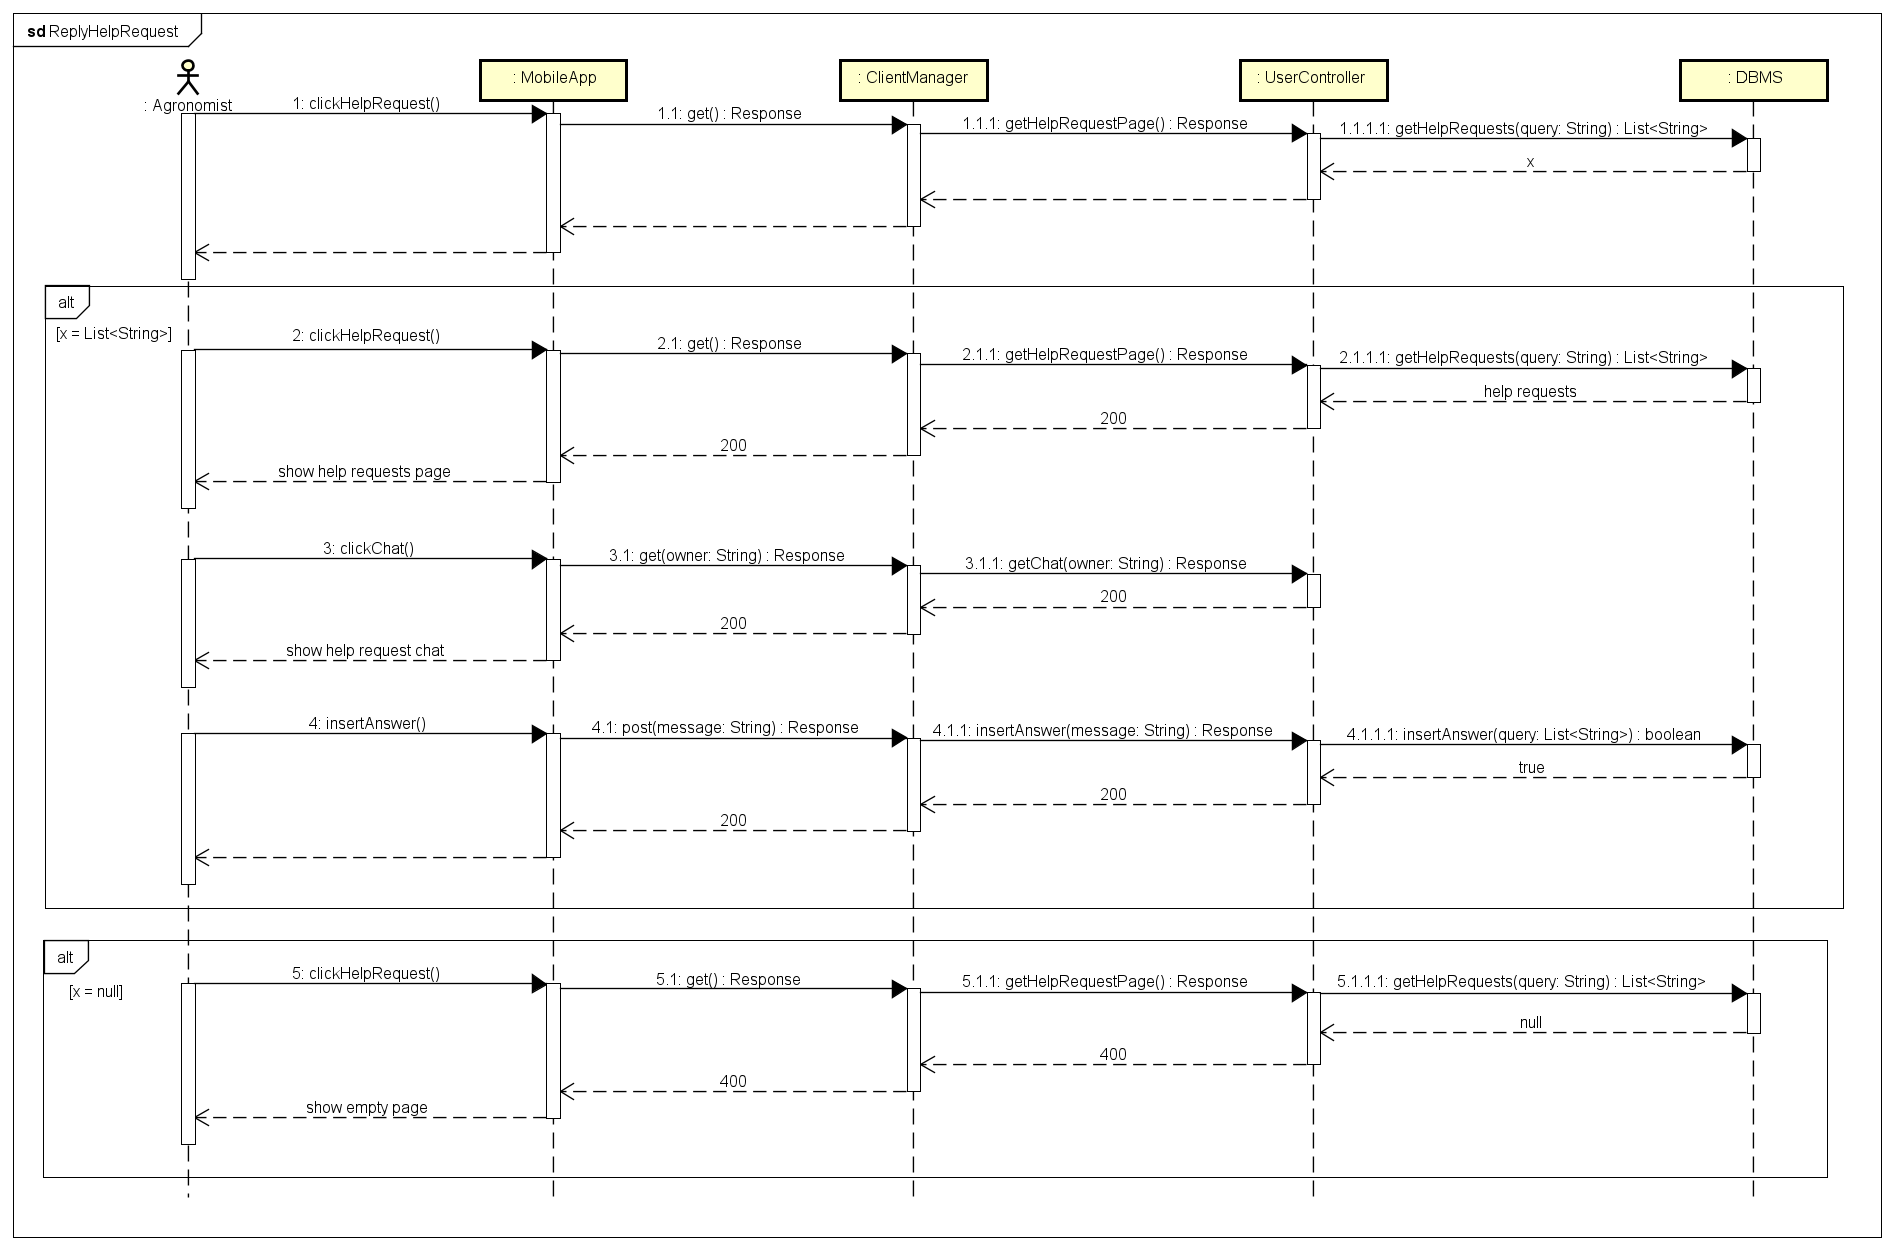
\includegraphics[width=\textwidth]{Images/SequenceDiagrams/ReplyHelpRequestDD.png}
    \end{center}
\end{figure}

This sequence diagram represents an operation that could be done only by agronomists.\\
After the user has clicked on the "Help Request" icon, the UserController queries the DBMS 
all the help requests submitted to the agronomist and shows them to him.\\
The user presses on a chat and enters his answer, which the UserController then inserts 
in the DBMS and sends a 200 response's status code to the Agronomist.\\
The UserController sends a 400 response's status code to the User only 
if there aren't help requests in the DBMS thus showing an empty page.


\newpage
\subsubsection{Insert Data}

\begin{figure}[H]
    \begin{center}
        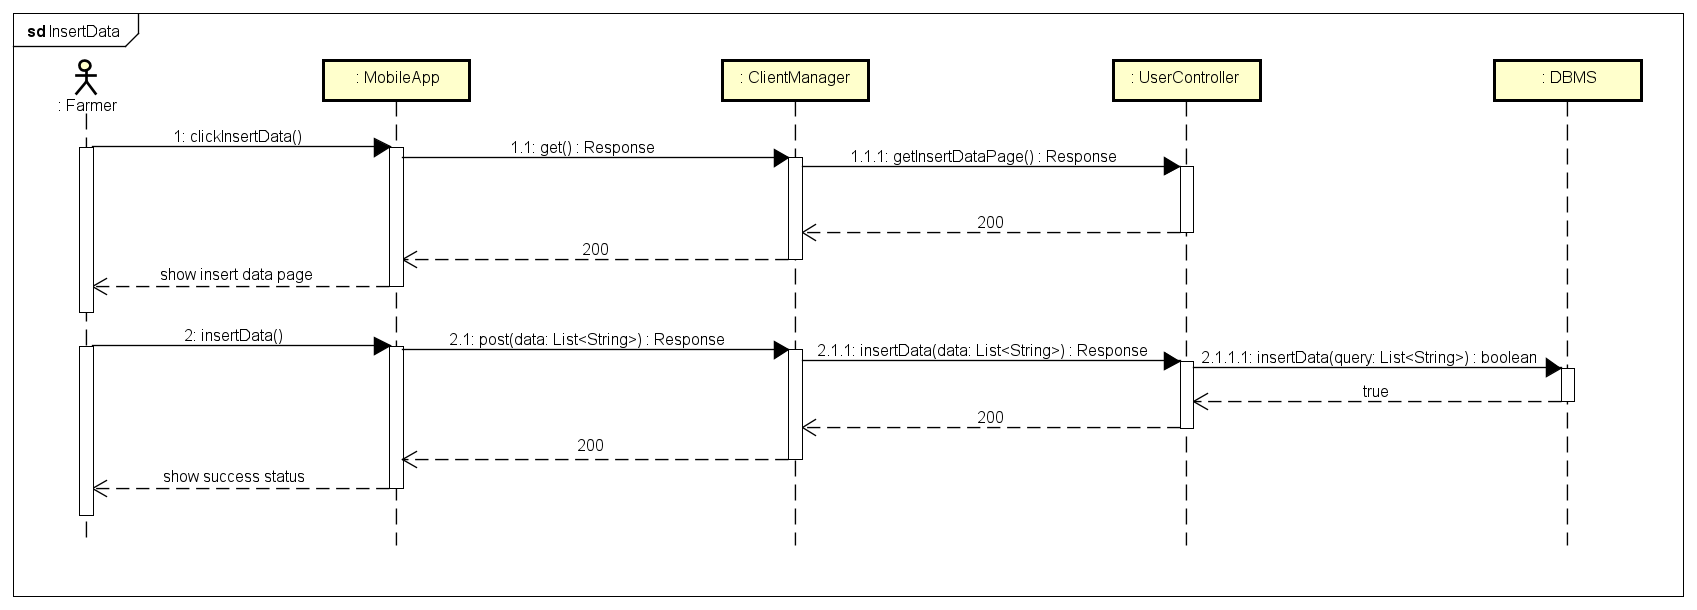
\includegraphics[width=\textwidth]{Images/SequenceDiagrams/InsertDataDD.png}
    \end{center}
\end{figure}

This sequence diagram represents an operation that could be done only by farmers.\\
After the User has entered the data concerning the crops of his farm, the UserController 
inserts these data in the DBMS and sends a 200 response's status code to the Farmer.


\bigskip
\subsubsection{Insert Threshold}

\begin{figure}[H]
    \begin{center}
        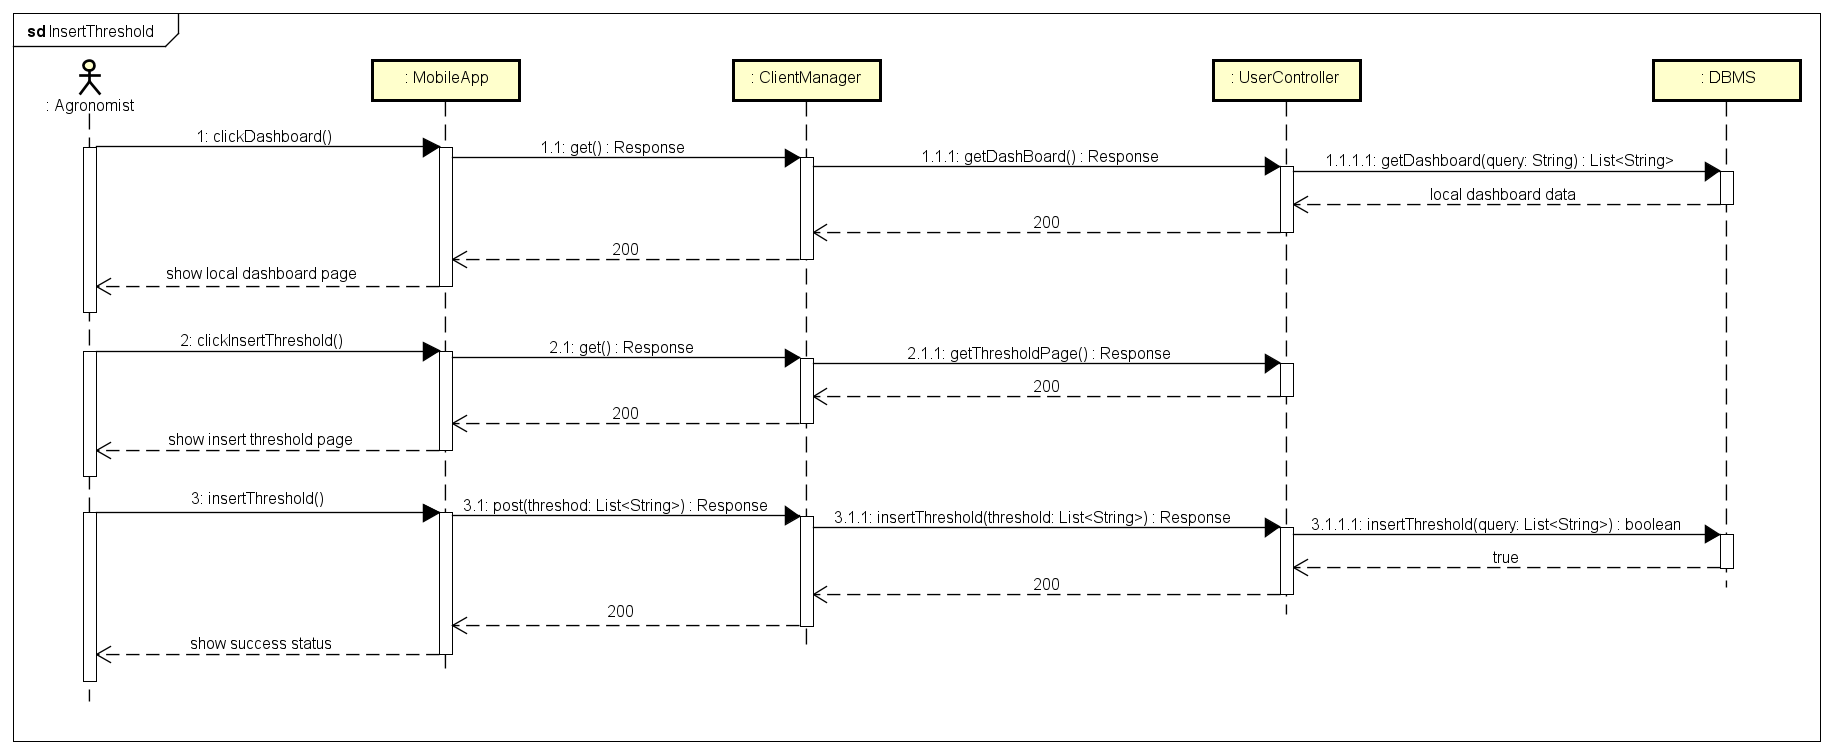
\includegraphics[width=\textwidth]{Images/SequenceDiagrams/InsertThresholdDD.png}
    \end{center}
\end{figure}

This sequence diagram represents the operation of inserting a threshold by agronomists.\\
From the Dashboard page, the Agronomist presses the "Insert Threshold" button and then inserts the threshold he deems appropriate.\\
After that, the UserController inserts the threshold in the DBMS and sends a 200 response's status to the Agronomist.


\newpage
\subsubsection{Personalized Suggestions}

\begin{figure}[H]
    \begin{center}
        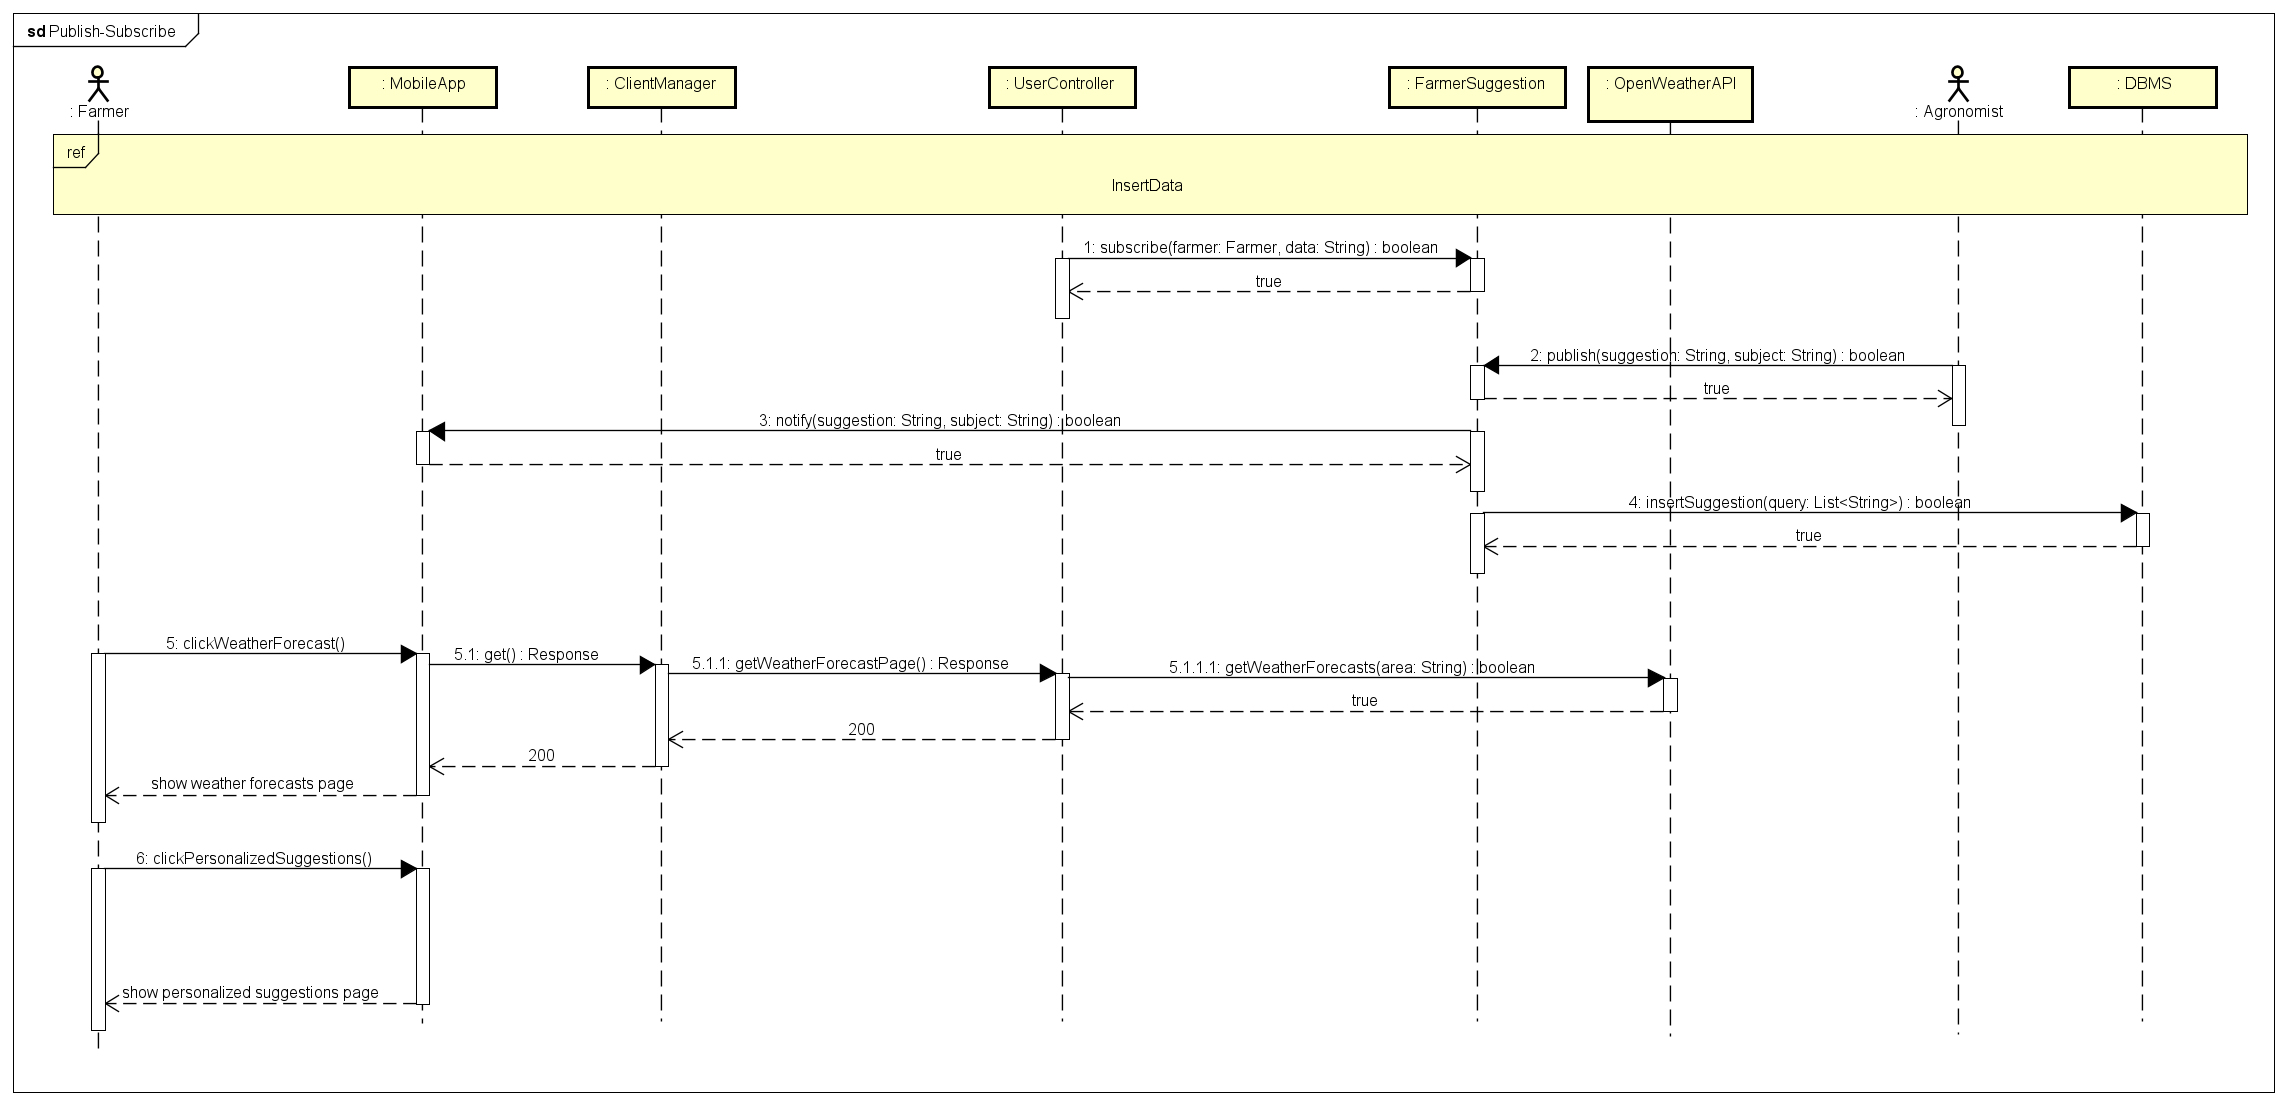
\includegraphics[width=\textwidth]{Images/SequenceDiagrams/Publish-SubscribeDD.png}
    \end{center}
\end{figure}

This sequence diagram represents how the forwarding of personalized suggestions to farmers works.\\
After having completed the operation of entering data concerning the crops, the UserController contacts 
the FarmerSuggestion to automatically subscribe the User to receive suggestions on how to improve their production.\\
Then when an agronomist inserts a suggestion through the FarmerSuggestion, the latter will 
forward the suggestion to all the farmers who had been subscribed.\\
Farmers can then find all their personalized suggestions by pressing the "Personalized Suggestions" button on the Weather Forecasts Page.


\newpage
\subsubsection{Logout}

\begin{figure}[H]
    \begin{center}
        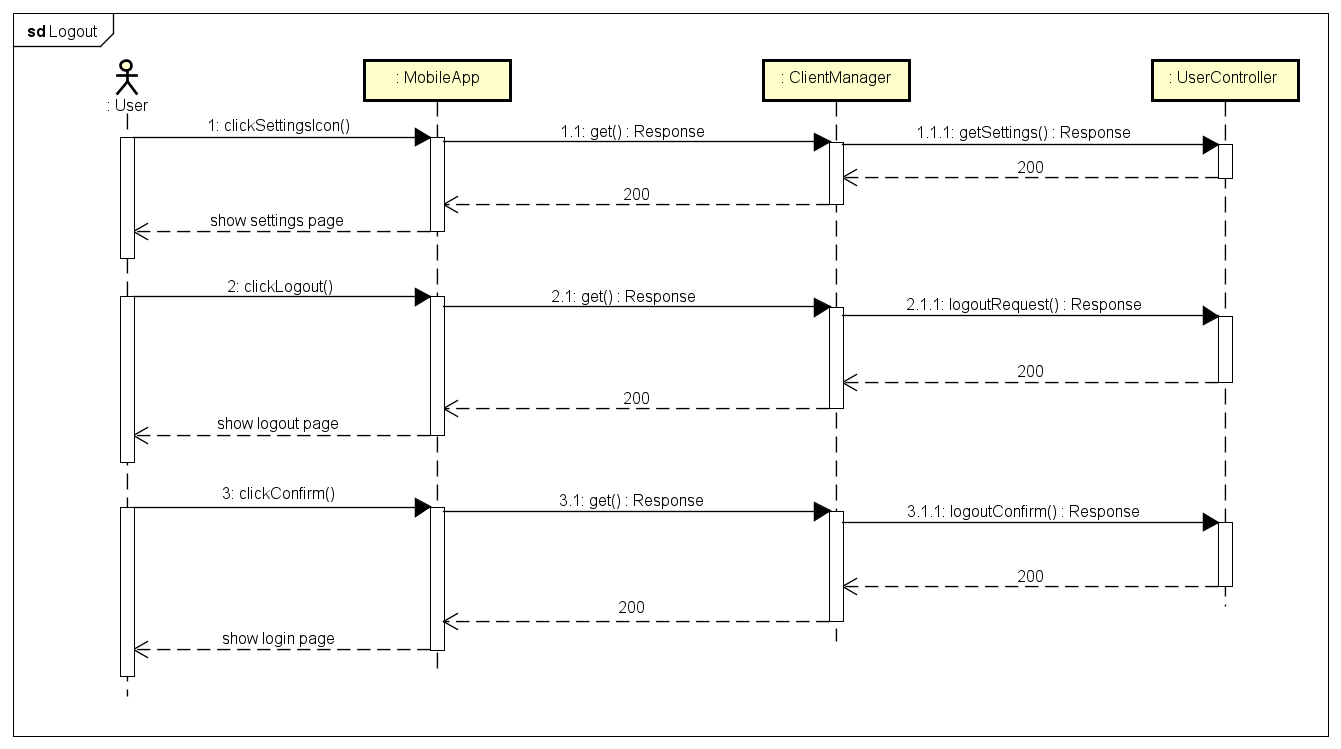
\includegraphics[width=\textwidth]{Images/SequenceDiagrams/LogoutDD.png}
    \end{center}
\end{figure}

The user clicks on the "Settings" icon and after on the "Logout" button. \\
The UserController asks the User if he is sure he wants to logout and after confirmation takes him to the login page.


\newpage

\subsection{Component Interfaces}
\begin{figure}[H]
    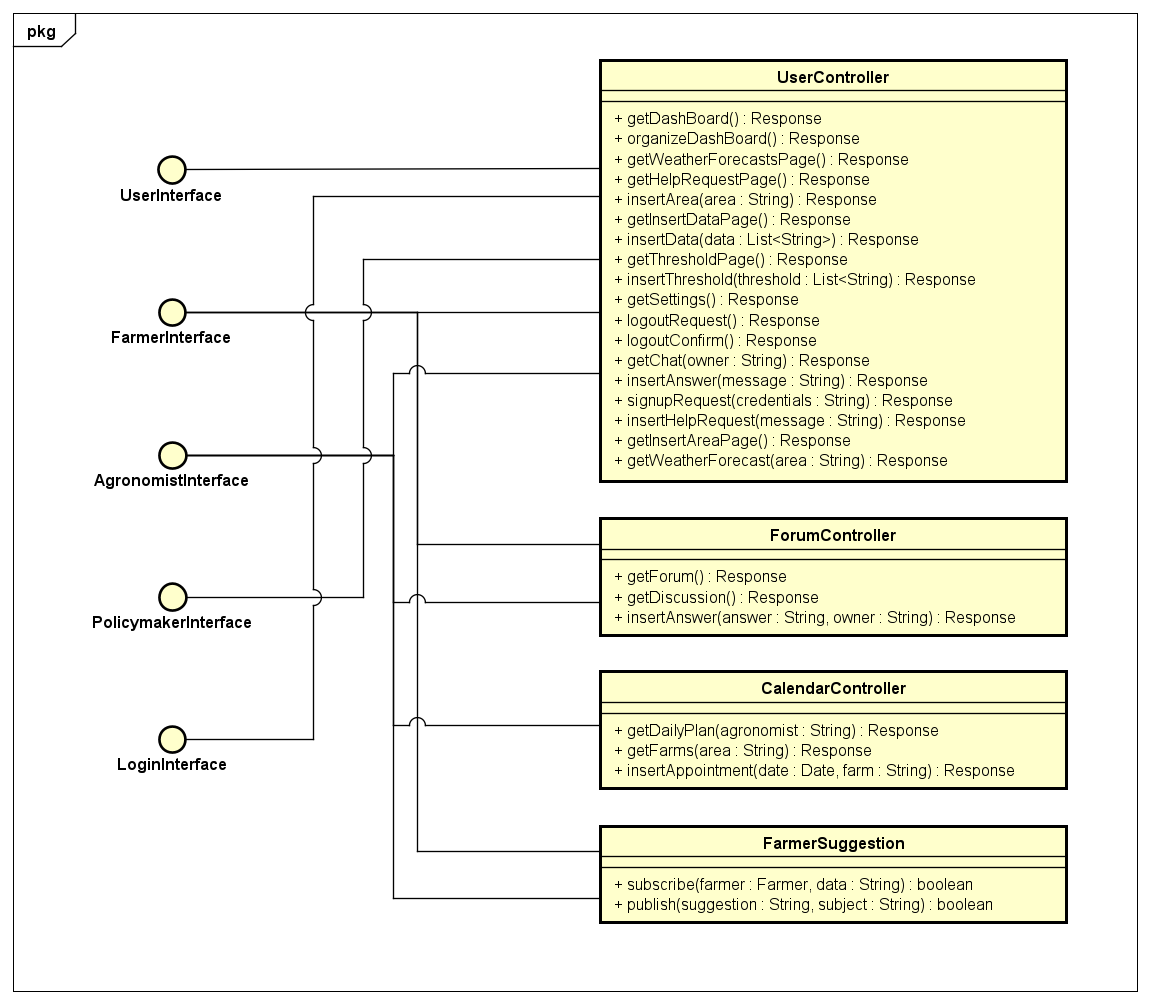
\includegraphics[width=\textwidth,height=\textheight,keepaspectratio]{Images/InterfaceDiagram.png}
    \caption{Interface Diagram}
    \label{fig:interface_diagram}
\end{figure}
Figure \ref{fig:interface_diagram} shows the main interfaces of the system.\newline
The \textbf{UserInterface} provides the functionalities common to all users, it is realized through just one controller the \textbf{UserController}. \newline
The \textbf{FarmerInterface} provides all the specific functionalities of the farmer and it is realized through three controllers: \textbf{UserController}, \textbf{ForumController}, \textbf{FarmerSuggestion}.\newline
The \textbf{AgronomistInterface} provides all the specific functionalities of the agronomist and it is realized through four controllers     :
\textbf{UserController}, \textbf{ForumController}, \textbf{FarmerSuggestion},\textbf{CalendarController}.\newline
The \textbf{PolicymakerInterface} provides all the specific functionalities of the policymaker and it is realized through one controller:
\textbf{UserController}.\newline
The \textbf{LoginInterface} provides all the functionalities for login and signup and it is realized through \textbf{UserController}.


\subsection{Logical Description of Data}
\begin{figure}[H]
    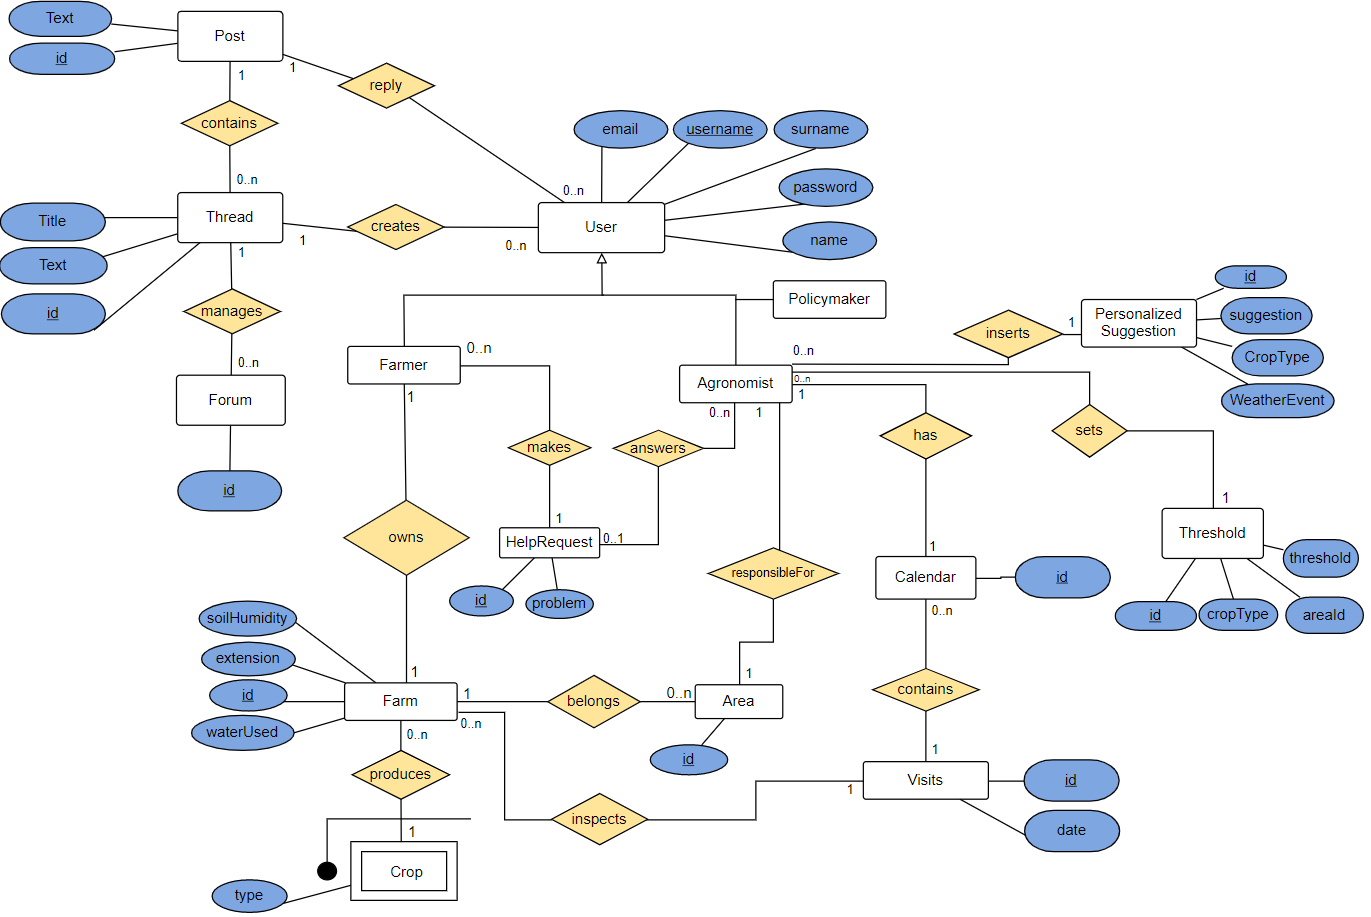
\includegraphics[width=\textwidth,height=\textheight,keepaspectratio]{Images/erDiagram.png}
    \caption{ER Diagram}
    \label{fig:er_diagram}
\end{figure}
Figure \ref{fig:er_diagram} shows a logical representation of the data that will be stored in the database of the system.


\bigskip
\subsection{Architectural Style and Patterns}
\subsubsection{Four-tiered architecture}
We chose this architecture for many reasons:
\begin{itemize}
    \item \textbf{Flexibility:} all parts of the application can be updated independently.
    \item \textbf{Load Distribution:} a 4-tier application enables replication in each tier: replicated application servers, through the exploitation of
    a load balancer, guarantee the avoidance of requests bottlenecks.
    \item \textbf{Scalability:} an application divided into several tiers allows developers to scale the architecture only for the most critical components.
\end{itemize}

\subsubsection{RESTful Architecture}
The \textbf{RESTful architecture} is based on HTTP and adopted both on the mobile and web sides. It is stateless so the server doesn't know anything
about the state of the client. \newline
An interesting constraint of this architecture is the code on demand, which gives the possibility of sending code to the client, where it is
executed locally. The application is intended to support \emph{client-side scripting}, which means that all requests and updates of the page are
made on client-side.

\subsubsection{Model View Controller (MVC)}
\textbf{Model–view–controller (MVC)} is a software design pattern commonly used for developing user interfaces that divide the related program logic into three
interconnected elements:
\begin{itemize}
    \item \textbf{Model:} it is the core component of the pattern. It is responsible for managing the data of the application. It receives user input from the controller.
    \item \textbf{View:} renders a presentation of the model in a particular format.
    \item \textbf{Controller:} accepts input and converts it to commands for the model or view.
\end{itemize}

\subsubsection{Publish-subscribe Architecture}
\textbf{Publish–subscribe} is a messaging pattern where senders of messages, called publishers, do not program the messages to be sent directly to specific receivers, called
subscribers, but instead categorize published messages into classes without knowledge of which subscribers if any, there may be. Similarly, subscribers express interest
in one or more classes and only receive messages that are of interest, without knowledge of which publishers, if any, there are. The application is intended to exploit the
\emph{topic-based} message filtering in which messages are published to "topics" or named logical channels: subscribers will receive all messages published to the topics to which
they subscribe, the publisher is responsible for defining the topics to which subscribers can subscribe.


\bigskip
\subsection{Other Design Decisions}
\subsubsection{Scale-Out}
As said before, the application is intended to be scaled out through the replication of nodes that are expected to generate bottlenecks. As shown in figure \ref{fig:architectue_diagram},
this approach requires load balancers to redirect the requests to nodes with the lowest workload.

\subsubsection{Thin client and Server}
The web application will be the \emph{thin client}: that's because the application is intended to keep as low information as possible on the client-side. This means that all the business
logic resides on the server, so a stable connection is required between the parts. The advantage of that is the low computational power required on the client-side.